\documentclass[xcolor={dvipsnames},aspectratio=169,10pt]{beamer}
\usetheme{mx}
\usepackage{graphicx}
\graphicspath{{figures/}}
%% utility packages
\usepackage{etoolbox}
\usepackage{multicol}
\usepackage{relsize}
\usepackage{fontawesome}

% better text justifying
\usepackage{microtype}
% justify text inside list environment
% Ref: http://liam0205.me/2017/04/11/justifying-in-beamer-s-lists/
\usepackage{ragged2e}
\makeatletter
\patchcmd{\itemize}{\raggedright}{\justifying}{}{}
\patchcmd{\beamer@enum@}{\raggedright}{\justifying}{}{}
\patchcmd{\@@description}{\raggedright}{\justifying}{}{}
\makeatother

% table of content with numbers and justification
% https://tex.stackexchange.com/questions/188773
\setbeamertemplate{section in toc}{\hspace*{1em}\inserttocsectionnumber.~\inserttocsection\par}
\setbeamertemplate{subsection in toc}{\hspace*{2em}\inserttocsectionnumber.\inserttocsubsectionnumber.~\inserttocsubsection\par}

% math related packages
\usepackage{amsmath}
\usepackage[ruled,vlined]{algorithm2e}
\SetAlCapNameFnt{\scriptsize}
\SetAlCapFnt{\scriptsize}
\SetAlFnt{\scriptsize}

% figure related packages
\usepackage{graphicx}
\usepackage[scale=2]{ccicons}
\usepackage{qrcode}
\usepackage{tikz}
\usepackage{tikzpagenodes}
\usetikzlibrary{positioning}

% table related packages
\usepackage{array}
\usepackage{booktabs}
\usepackage{multirow}
\usepackage{colortbl}
\newcommand{\tabincell}[2]{\begin{tabular}{@{}#1@{}}#2\end{tabular}}

% code highlight
\usepackage{listings}
%\usepackage{minted}
%\definecolor{mintedbg}{HTML}{E5E9F0}
%\setminted{autogobble,bgcolor=mintedbg,fontsize=\small}
%\setmintedinline{bgcolor=mintedbg,fontsize=\smaller}
%\newminted{bash}{}
%\newminted{latex}{}
%\newmintinline{bash}{}
%\newmintinline{latex}{}
%\newcommand{\texdoc}[2]{\href{#2}{\bashinline|texdoc #1|}}

% hyperref setting
\hypersetup{
  unicode,
  psdextra,
  bookmarksnumbered=true,
  bookmarksopen=true,
  bookmarksopenlevel=3,
  bookmarksdepth=4,
  pdfcenterwindow=true,
  pdfstartview={Fit},
  pdfpagemode={FullScreen},
  pdfpagelayout={SinglePage},
}
\usepackage{bookmark}

% beamer theme
\usetheme{metropolis}
\metroset{block=fill,numbering=fraction}

% caption style
\usepackage{subcaption}
\setlength\abovecaptionskip{3pt}
\setbeamerfont{caption}{size=\scriptsize}
\renewcommand{\figurename}{Fig.}
\captionsetup{labelformat=empty,labelsep=none,textfont={bf,it}}

% Ref: https://github.com/gpoore/minted/blob/master/source/minted.dtx
\newenvironment{latexexample}
{\VerbatimEnvironment\begin{VerbatimOut}[gobble=3]{example.out}}{\end{VerbatimOut}%
  \begin{center}
    \begin{minipage}{0.47\linewidth}%
      \inputminted[resetmargins,fontsize=\scriptsize]{latex}{example.out}%
    \end{minipage}%
    \hspace{0.05\linewidth}%
    \begin{minipage}{0.47\linewidth}%
      \begin{framed}
        \setlength{\parindent}{2em}%
        \input{example.out}%
      \end{framed}
    \end{minipage}%
  \end{center}
}

\newenvironment{mathexample}
{\VerbatimEnvironment\begin{VerbatimOut}[gobble=3]{example.out}}{\end{VerbatimOut}%
  \begin{center}
    \begin{minipage}{0.47\linewidth}%
      \inputminted[resetmargins,fontsize=\scriptsize]{latex}{example.out}%
    \end{minipage}%
    \hspace{0.05\linewidth}%
    \begin{minipage}{0.47\linewidth}%
      \begin{framed}
        \[ \input{example.out} \]
      \end{framed}
    \end{minipage}%
  \end{center}
}

\newenvironment{mathexamples}
{\VerbatimEnvironment\begin{VerbatimOut}[gobble=3]{example.out}}{\end{VerbatimOut}%
  \begin{center}
    \begin{minipage}{0.47\linewidth}%
      \inputminted[resetmargins,fontsize=\scriptsize]{latex}{example.out}%
    \end{minipage}%
    \hspace{0.05\linewidth}%
    \begin{minipage}{0.47\linewidth}%
      \begin{framed}
        \directlua{
          local first = true
          for line in io.lines('example.out') do
          if first then
          first = false
          else
          tex.print('\\newline ')
          end
          tex.print('$' .. line .. '$')
          end
        }
      \end{framed}
    \end{minipage}%
  \end{center}
}



%---------------------------------------------------------------------
% Add Paper using {\paper{}. begin{beawer} ... end{beamer} }
%---------------------------------------------------------------------
\newcommand\paper[1]{
	\setbeamertemplate{footline}
	{
		\begin{beamercolorbox}[wd=\textwidth,ht=3mm,dp=03mm,leftskip=0.3cm,rightskip=0.3cm]{black}%
        		\usebeamerfont{page number in head/foot}
			(#1)\mbox{}\hfill\insertframenumber
		\end{beamercolorbox}%
	}
}



\title{  
Miguel Xochicale -- Introduction
% Miguel Xochicale: Past, present and future
%Tue 29 Nov 00:48:01 GMT 2022
} 

\subtitle{RSGD slides}

\author{
{\bf Miguel Xochicale, PhD} (\faTwitter @\_mxochicale  \faGithub @mxochicale)
}
\date{
%Workshop Presenting with Confidence \\
%January 27, 2021; 11h00m
\today
}
\institute{
	Advanced Research Computing Centre and WEISS \\
	Universtiy College London
	}

\titlegraphic{
  \begin{tikzpicture}[overlay, remember picture]
    \node[%
      above right=0.35cm and -0.2cm of current page footer area.south west,
      anchor=south west,
      inner sep=0pt] {%
      \usebeamerfont{footline}
      \begin{tabular}{lm{.8\textwidth}}
        \href{http://creativecommons.org/licenses/by/4.0/}{\ccby} &
        This slices is licensed under a
	\href{http://creativecommons.org/licenses/by/4.0/}
		{Creative Commons ``Attribution 4.0 International''} license. 
	\par Get source of this slides and see further references 
		from \url{https://github.com/mxochicale/ADDREPONAME}.
      \end{tabular}
    };
    \node[%
      above left=0.35cm and 0cm of current page footer area.south east,
      anchor=south east,
      inner sep=0pt]{\qrcode[height=1.5cm]{https://github.com/mxochicale/ADDREPONAME}};
  \end{tikzpicture}
}

\begin{document}

\maketitle

\begin{frame}
\frametitle{Table of Contents}
    \tableofcontents
\end{frame}

\section{My trajectory}

\begin{frame}
  \frametitle{Table of Contents}
  \tableofcontents[currentsection]
\end{frame}



%%%%%%%%%%%%%%%%%%%%%%%%%%%%%%%%%%%%%%%%%%%%%%%%%%%%%%%%
{
%\paper{Lastname N. YEAR in journal of...}
\begin{frame}{My trajectory}

  \begin{figure}
  \centering
  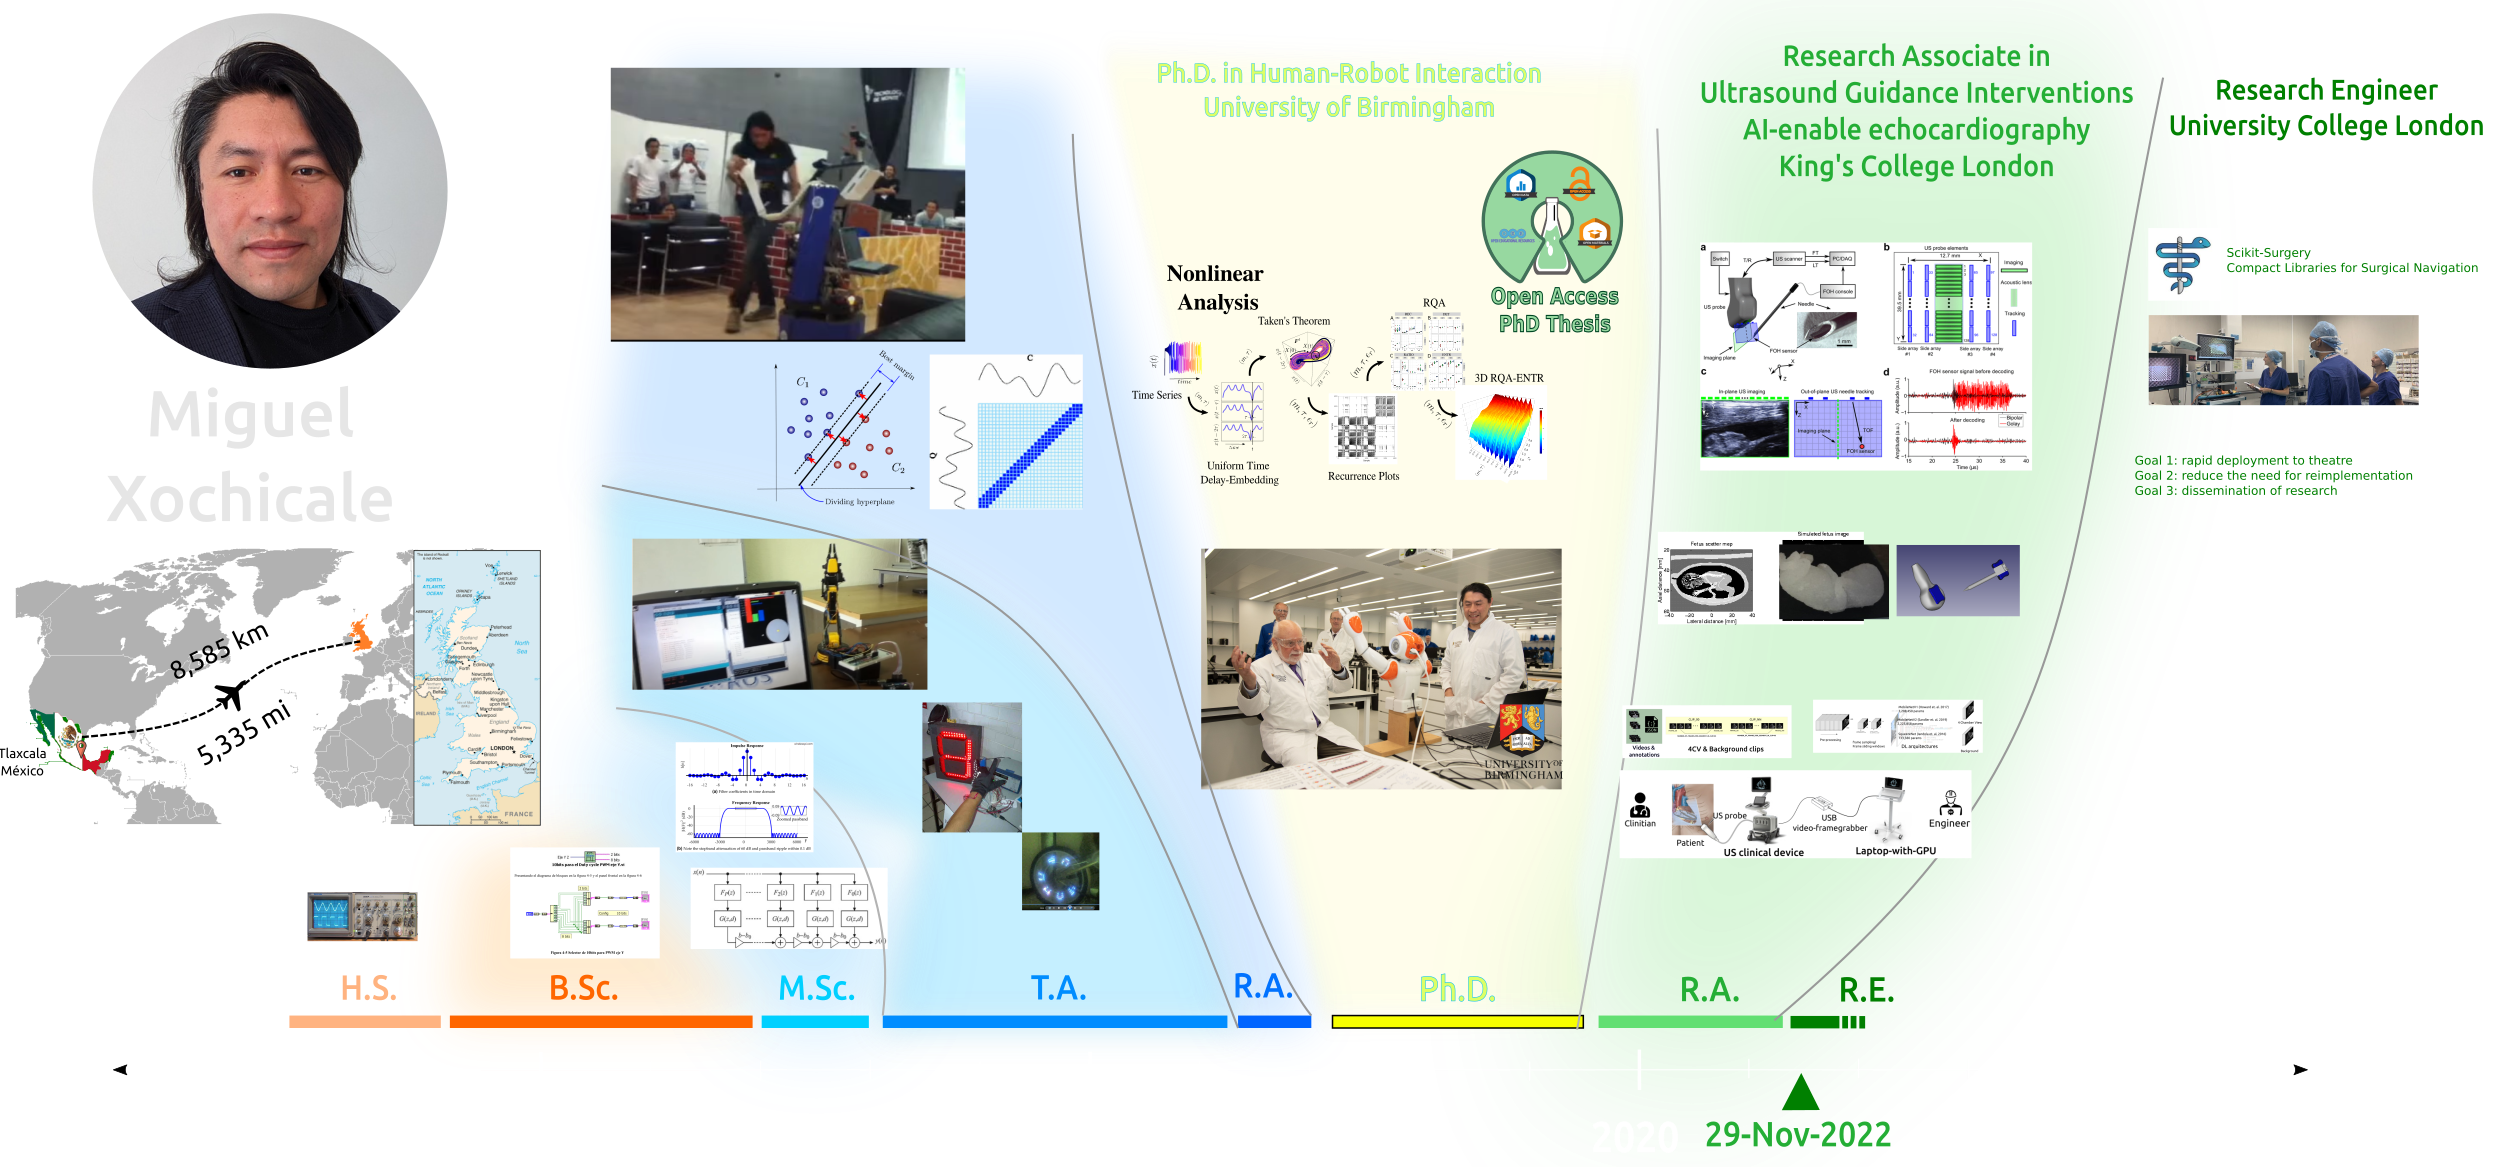
\includegraphics[width=1.0\textwidth]{miguel-xochicale/versions/drawing-v05}
  \end{figure}

\end{frame}
}



%%%%%%%%%%%%%%%%%%%%%%%%%%%%%%%%%%%%%%%%%%%%
\section{PhD in Human-Robot Interaction (2014-2019)}


\begin{frame}
      \frametitle{Table of Contents}
      \tableofcontents[currentsection]
  \end{frame}



% \subsection{Clinical background}

%%%%%%%%%%%%%%%%%%%%%%%%%%%%%%%%%%%%%%%%%%%%%%%%%%%%%%%%
{
\paper{
Xochicale Miguel, PhD thesis 2018; \url{https://github.com/mxochicale-phd}
}

\begin{frame}{PhD in Human-Robot Interaction (2014-2019) \\ University of Birmingham}
      \begin{figure}
        \centering
        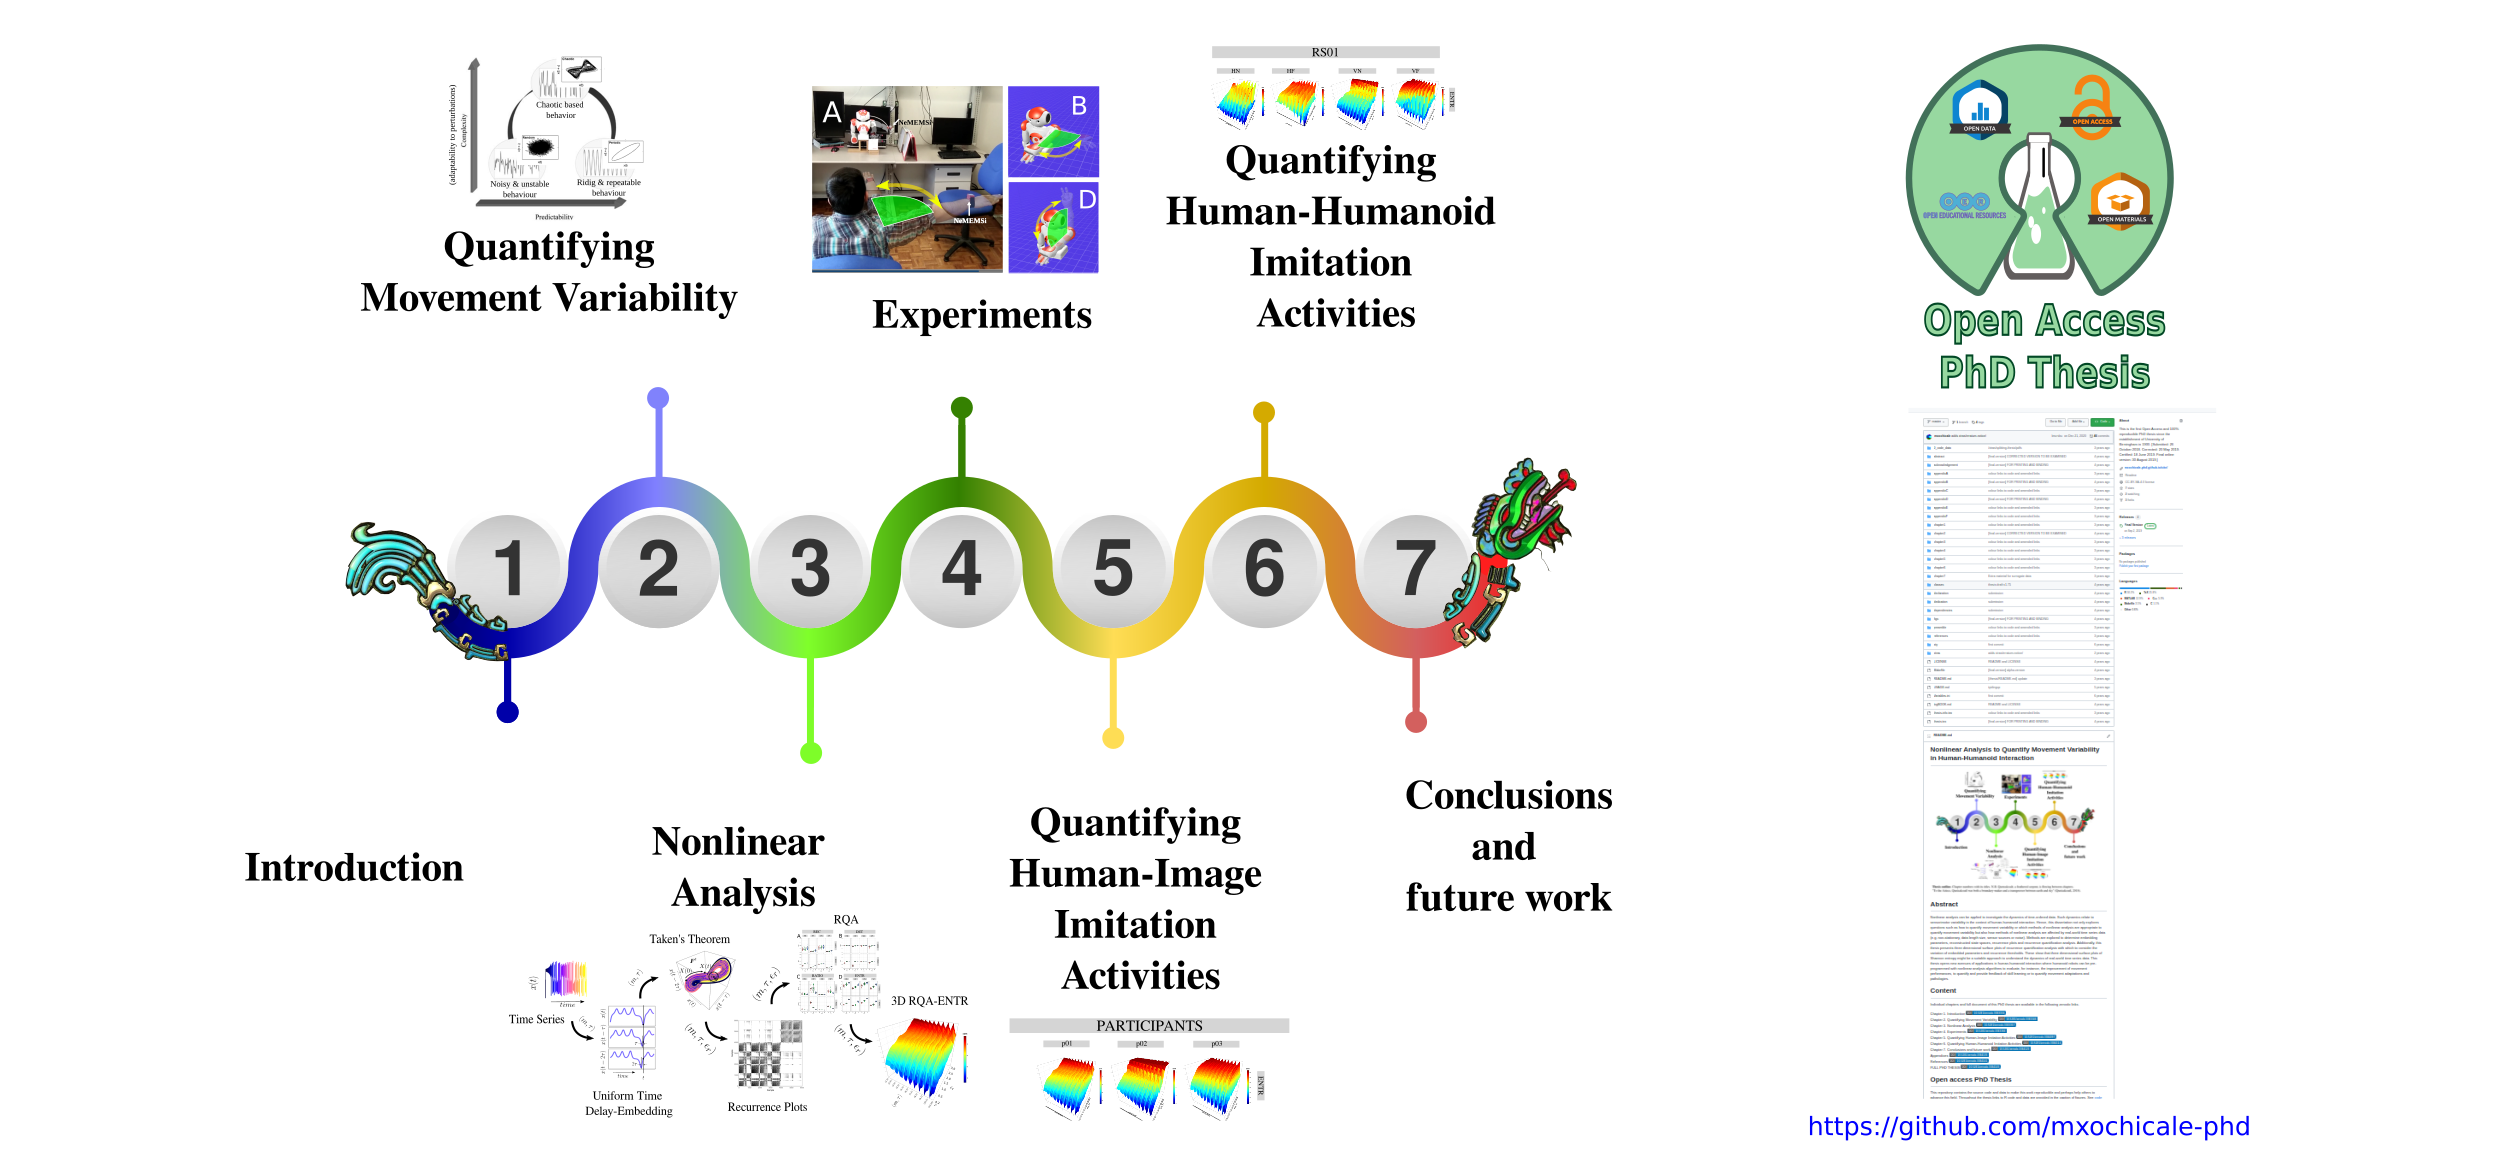
\includegraphics[width=1.0\textwidth]{phd-thesis-A/versions/drawing-v00}
        % \caption{The sonographer-probe-patient control system}
      \end{figure}
\end{frame}
}


%%%%%%%%%%%%%%%%%%%%%%%%%%%%%%%%%%%%%%%%%%%%%%%%%%%%%%%%
{
\paper{
Xochicale Miguel, PhD thesis 2018; \url{https://github.com/mxochicale-phd}
}

\begin{frame}{PhD in Human-Robot Interaction (2014-2019) \\ University of Birmingham}
      \begin{figure}
        \centering
        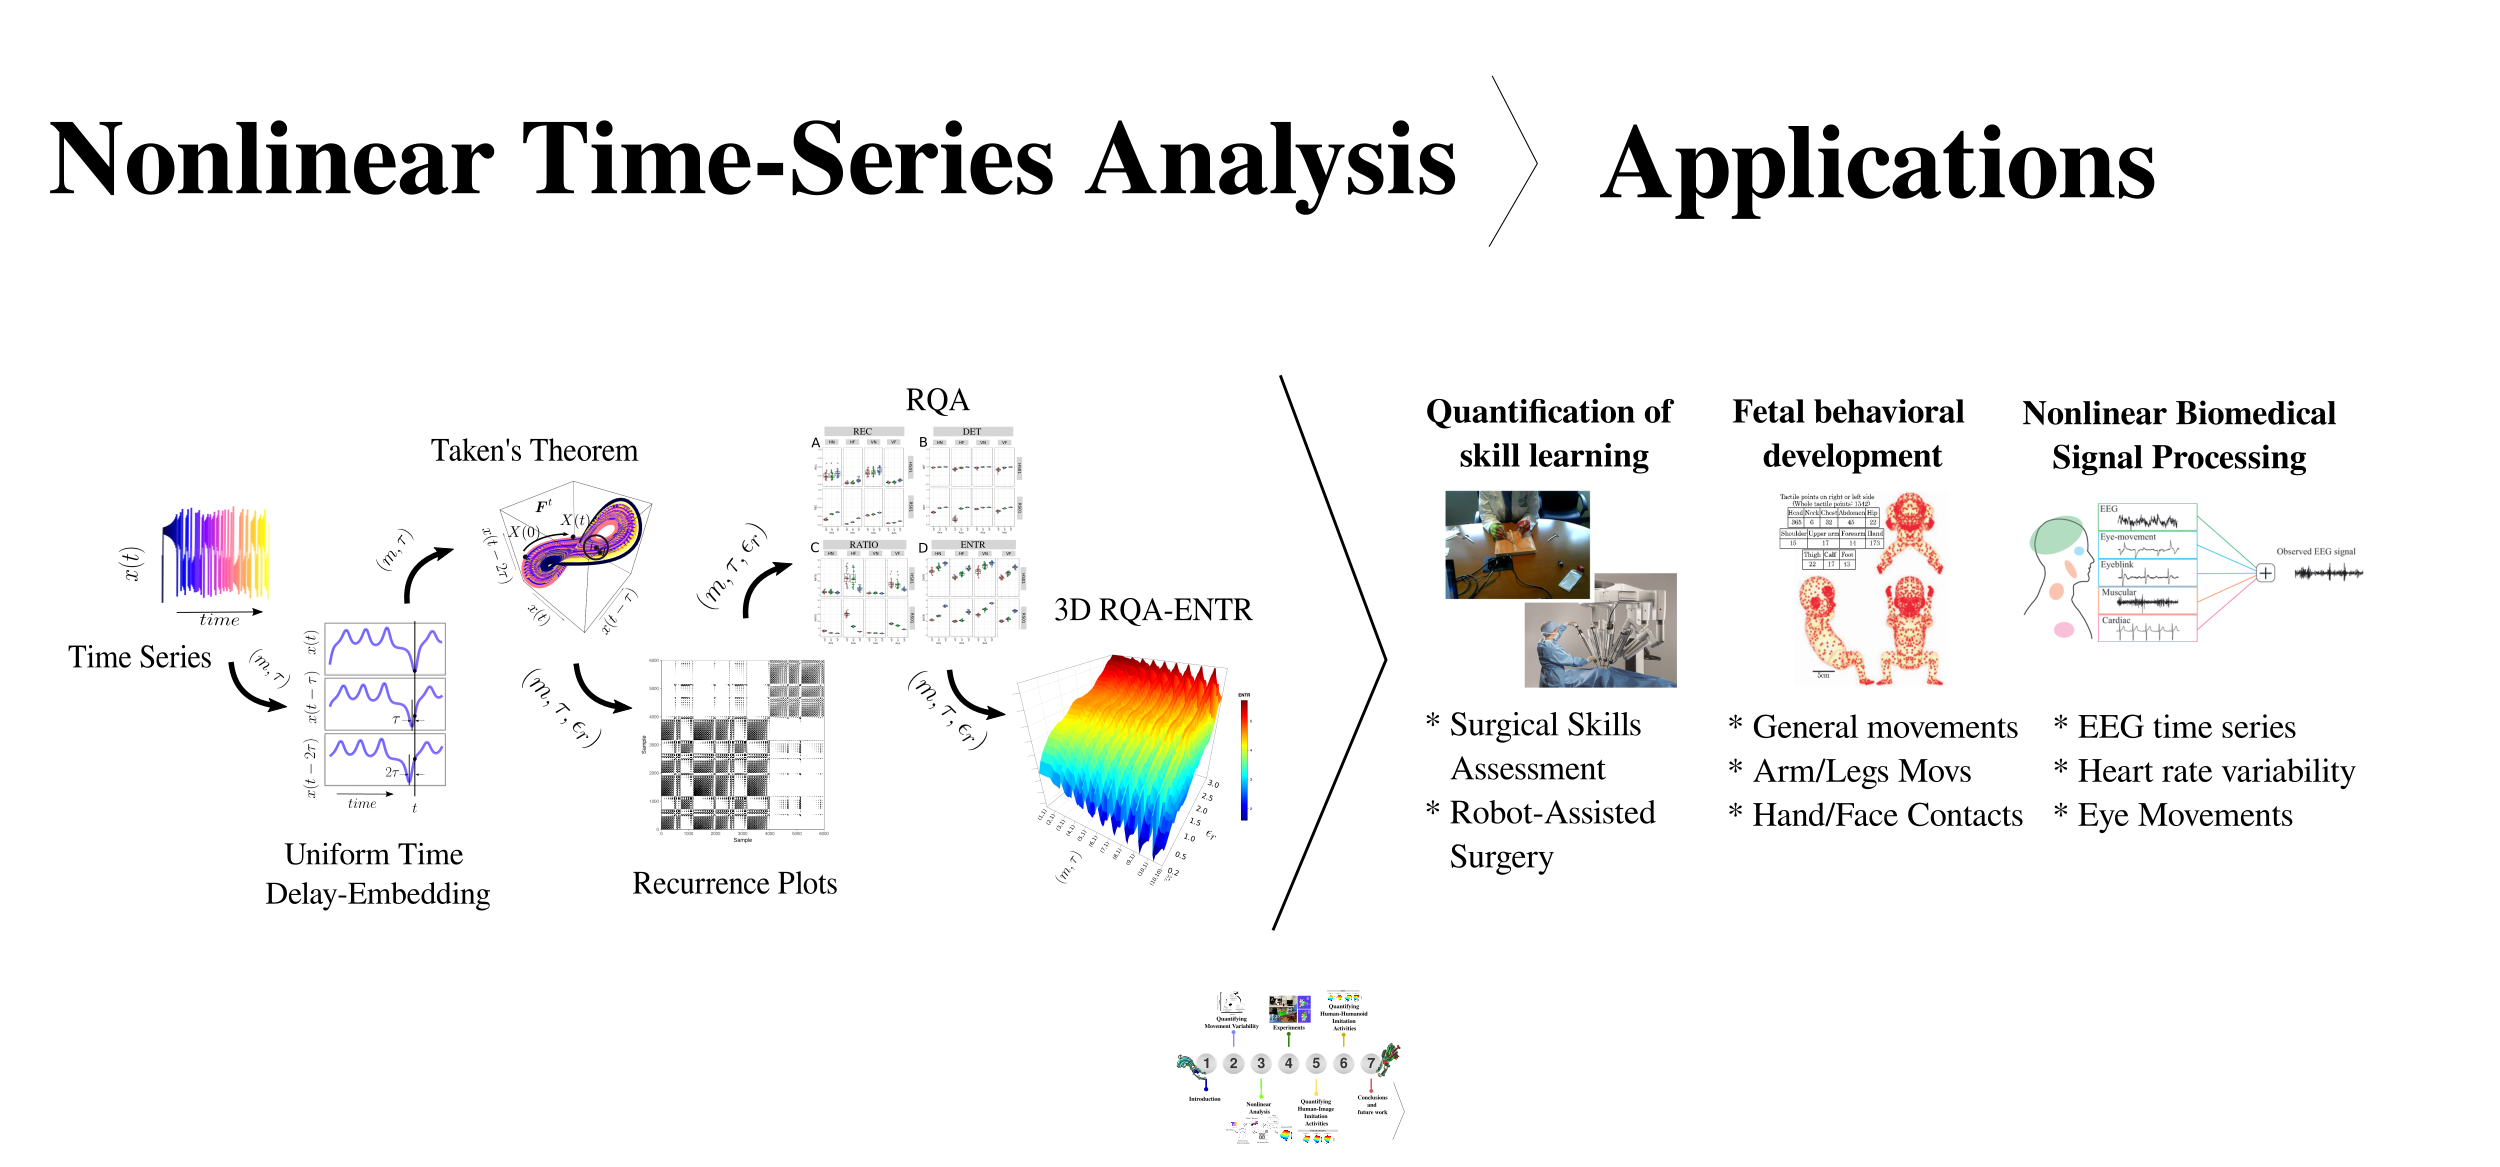
\includegraphics[width=1.0\textwidth]{phd-thesis-B/versions/drawing-v00}
        % \caption{The sonographer-probe-patient control system}
      \end{figure}
\end{frame}
}




%%%%%%%%%%%%%%%%%%%%%%%%%%%%%%%%%%%%%%%%%%%%
\section{Ultrasound Needle Tracking}


\begin{frame}
  \frametitle{Table of Contents}
  \tableofcontents[currentsection]
\end{frame}



% \subsection{Clinical background}

% %%%%%%%%%%%%%%%%%%%%%%%%%%%%%%%%%%%%%%%%%%%%%%%%%%%%%%%%
% {
% \paper{
% Wright-Gilbertson M. 2014 in PhD thesis; \url{https://en.wikipedia.org/wiki/Gestational_age}; 
% National-Health-Service 2021. Screening for down’s syndrome, edwards’ syndrome and patau’s syndrome. \url{https://www.nhs.uk/pregnancy/your-pregnancy-care} 
% }

% \begin{frame}{Dating US scan (12-week scan)}
%       \begin{figure}
%         \centering
%         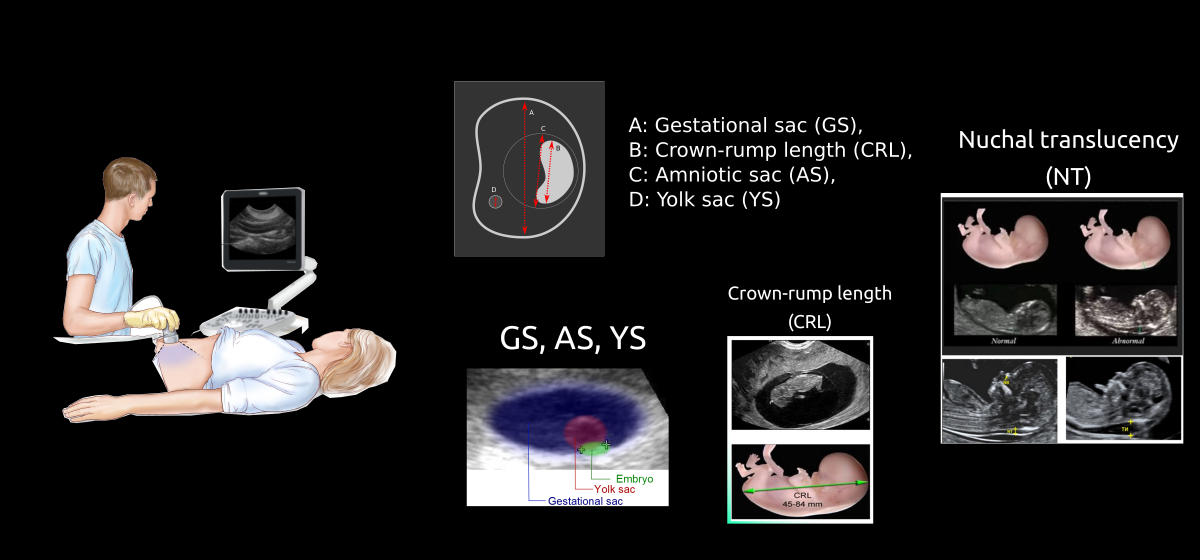
\includegraphics[width=1.0\textwidth]{12-week-scan/versions/drawing-v01}
%         % \caption{The sonographer-probe-patient control system}
%       \end{figure}
% \end{frame}
% }



%%%%%%%%%%%%%%%%%%%%%%%%%%%%%%%%%%%%%%%%%%%%%%%%%%%%%%%%
{
\paper{
  Baker, Christian; Xochicale, Miguel; et al. 
  % Fang-Yu Lin, Sunish Mathews, Francois Joubert, Dzhoshkun I. Shakir, Richard Miles, Charles A. Mosse, Tianrui Zhao, Weidong Liang, Yada Kunpalin, Brian Dromey, Talisa Mistry, Neil J. Sebire, Edward Zhang, Sebastien Ourselin, Paul C. Beard, Anna L. David, Adrien E. Desjardins, Tom Vercauteren, and Wenfeng Xia. 2022.
   "Intraoperative Needle Tip Tracking with an Integrated Fibre-Optic Ultrasound Sensor" Sensors 22, no. 23: 9035. https://doi.org/10.3390/s22239035
}
\begin{frame}{Intraoperative Needle Tip Tracking (2019-2021) @ KCL}
      \begin{figure}
        \centering
        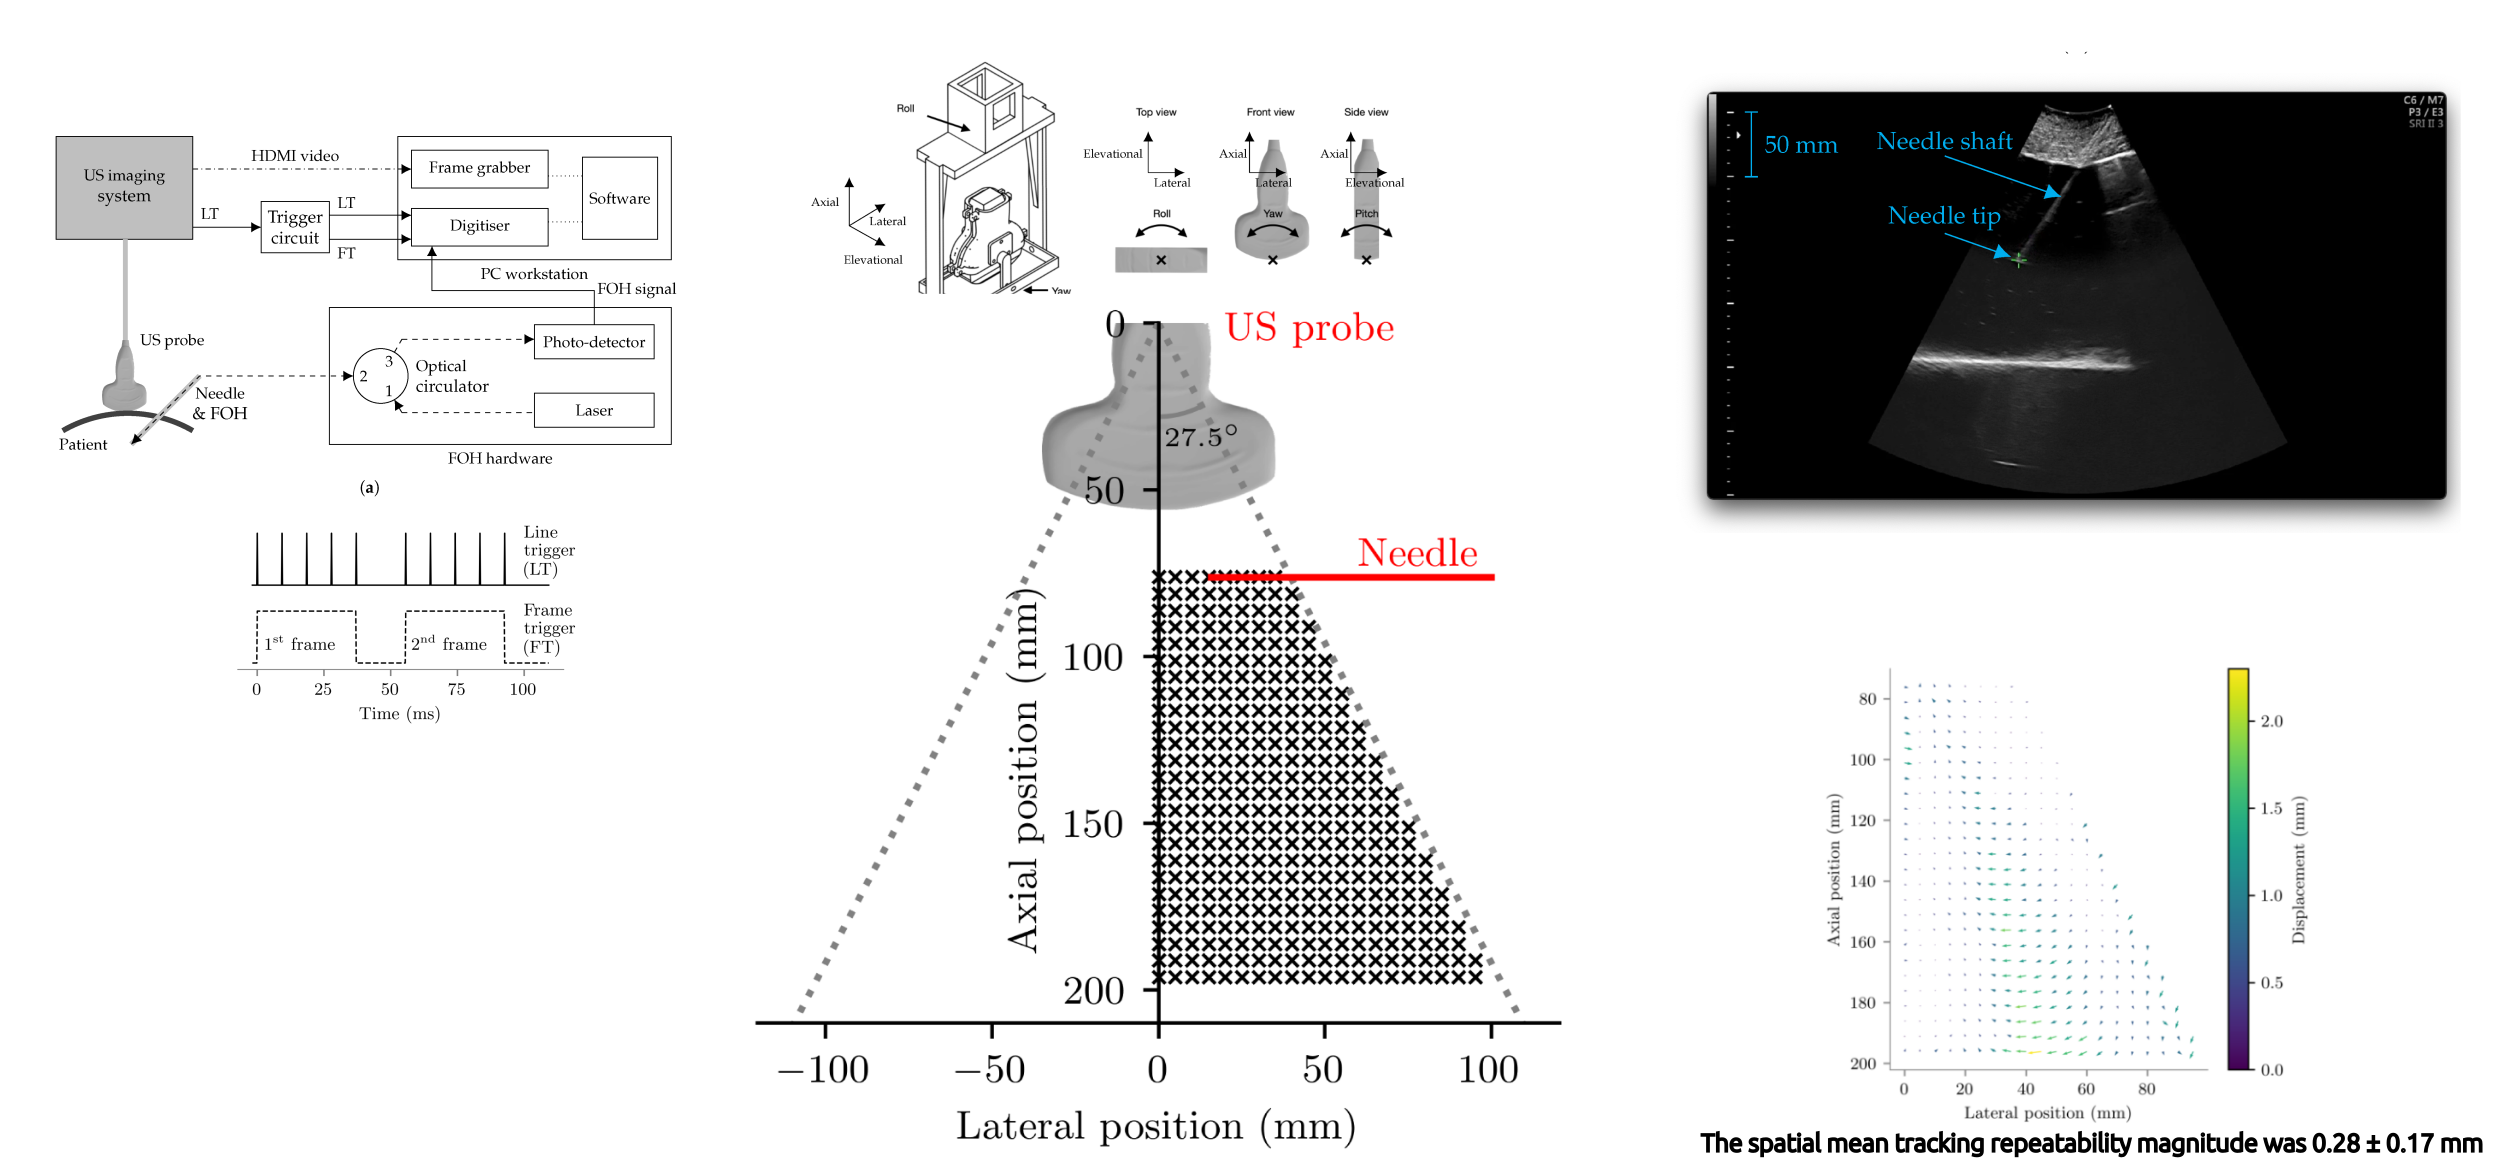
\includegraphics[width=1.0\textwidth]{unt/versions/drawing-v00}
        % \caption{The sonographer-probe-patient control system}
      \end{figure}
\end{frame}
}





%%%%%%%%%%%%%%%%%%%%%%%%%%%%%%%%%%%%%%%%%%%%%%%%%%%%%%%%
{
\paper{
  Xochicale Miguel et al. 
  Finding a fETus with UltraSound (FETUS); \faGithub    https://github.com/xfetus/pe 
}
\begin{frame}{Finding a fETus with UltraSound (FETUS) (2019-2021) @ KCL}
      \begin{figure}
        \centering
        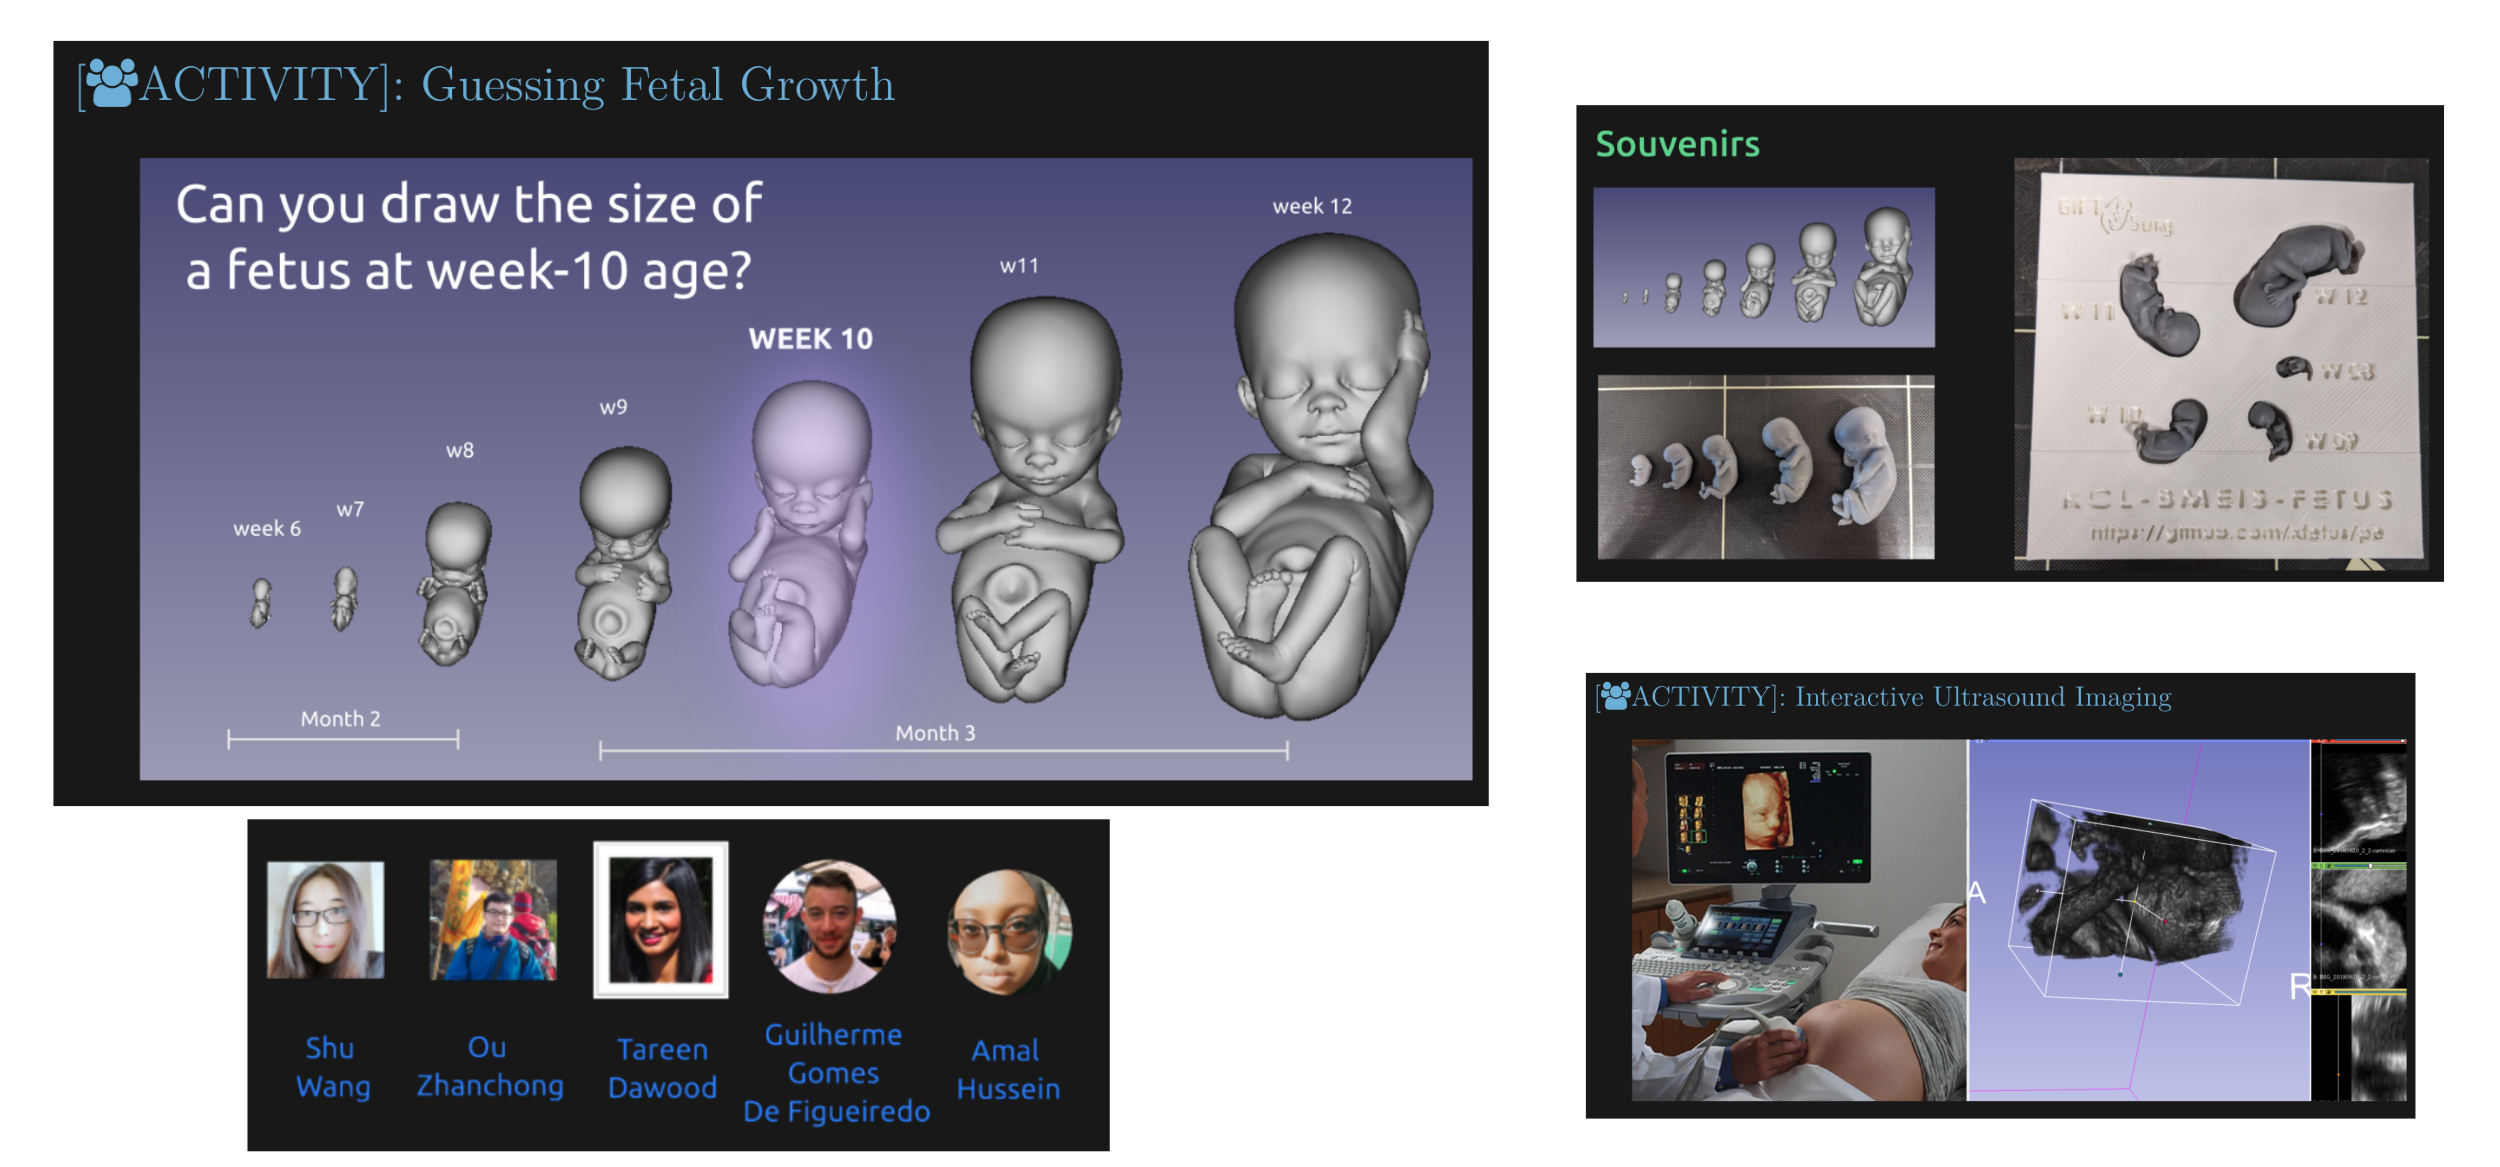
\includegraphics[width=1.0\textwidth]{fetus/versions/drawing-v00}
        % \caption{The sonographer-probe-patient control system}
      \end{figure}
\end{frame}
}






% \subsection{Research aims}


% %%%%%%%%%%%%%%%%%%%%%%%%%%%%%%%%%%%%%%%%%%%%%%%%%%%%%%%%
% {
% %\paper{Wright-Gilbertson M. 2014 in PhD thesis}
% \begin{frame}{Research aims}	
% \begin{itemize}
% \item Investigate and implement deep-learning methods for synthetic fetal ultrasound imaging of normal and abnormal cases;
% \item Propose and apply methods to evaluate quantitative and qualitative images to investigate fetal biomechanics; and 
% \item Design and  test fetal phantoms that mimic various poses, and fetal ages.
% % \item 
% \end{itemize}

% \end{frame}
% }



%%%%%%%%%%%%%%%%%%%%%%%%%%%%%%%%%%%%%%%%%%%%
\section{AI-enabled echocardiography}


\begin{frame}
      \frametitle{Table of Contents}
      \tableofcontents[currentsection]
  \end{frame}

% \subsection{Clinical background}

%%%%%%%%%%%%%%%%%%%%%%%%%%%%%%%%%%%%%%%%%%%%%%%%%%%%%%%%
{
% \paper{
% Wright-Gilbertson M. 2014 in PhD thesis; \url{https://en.wikipedia.org/wiki/Gestational_age}; 
% National-Health-Service 2021. Screening for down’s syndrome, edwards’ syndrome and patau’s syndrome. \url{https://www.nhs.uk/pregnancy/your-pregnancy-care} 
% }

\begin{frame}{The four-chamber view}
      \begin{figure}
        \centering
        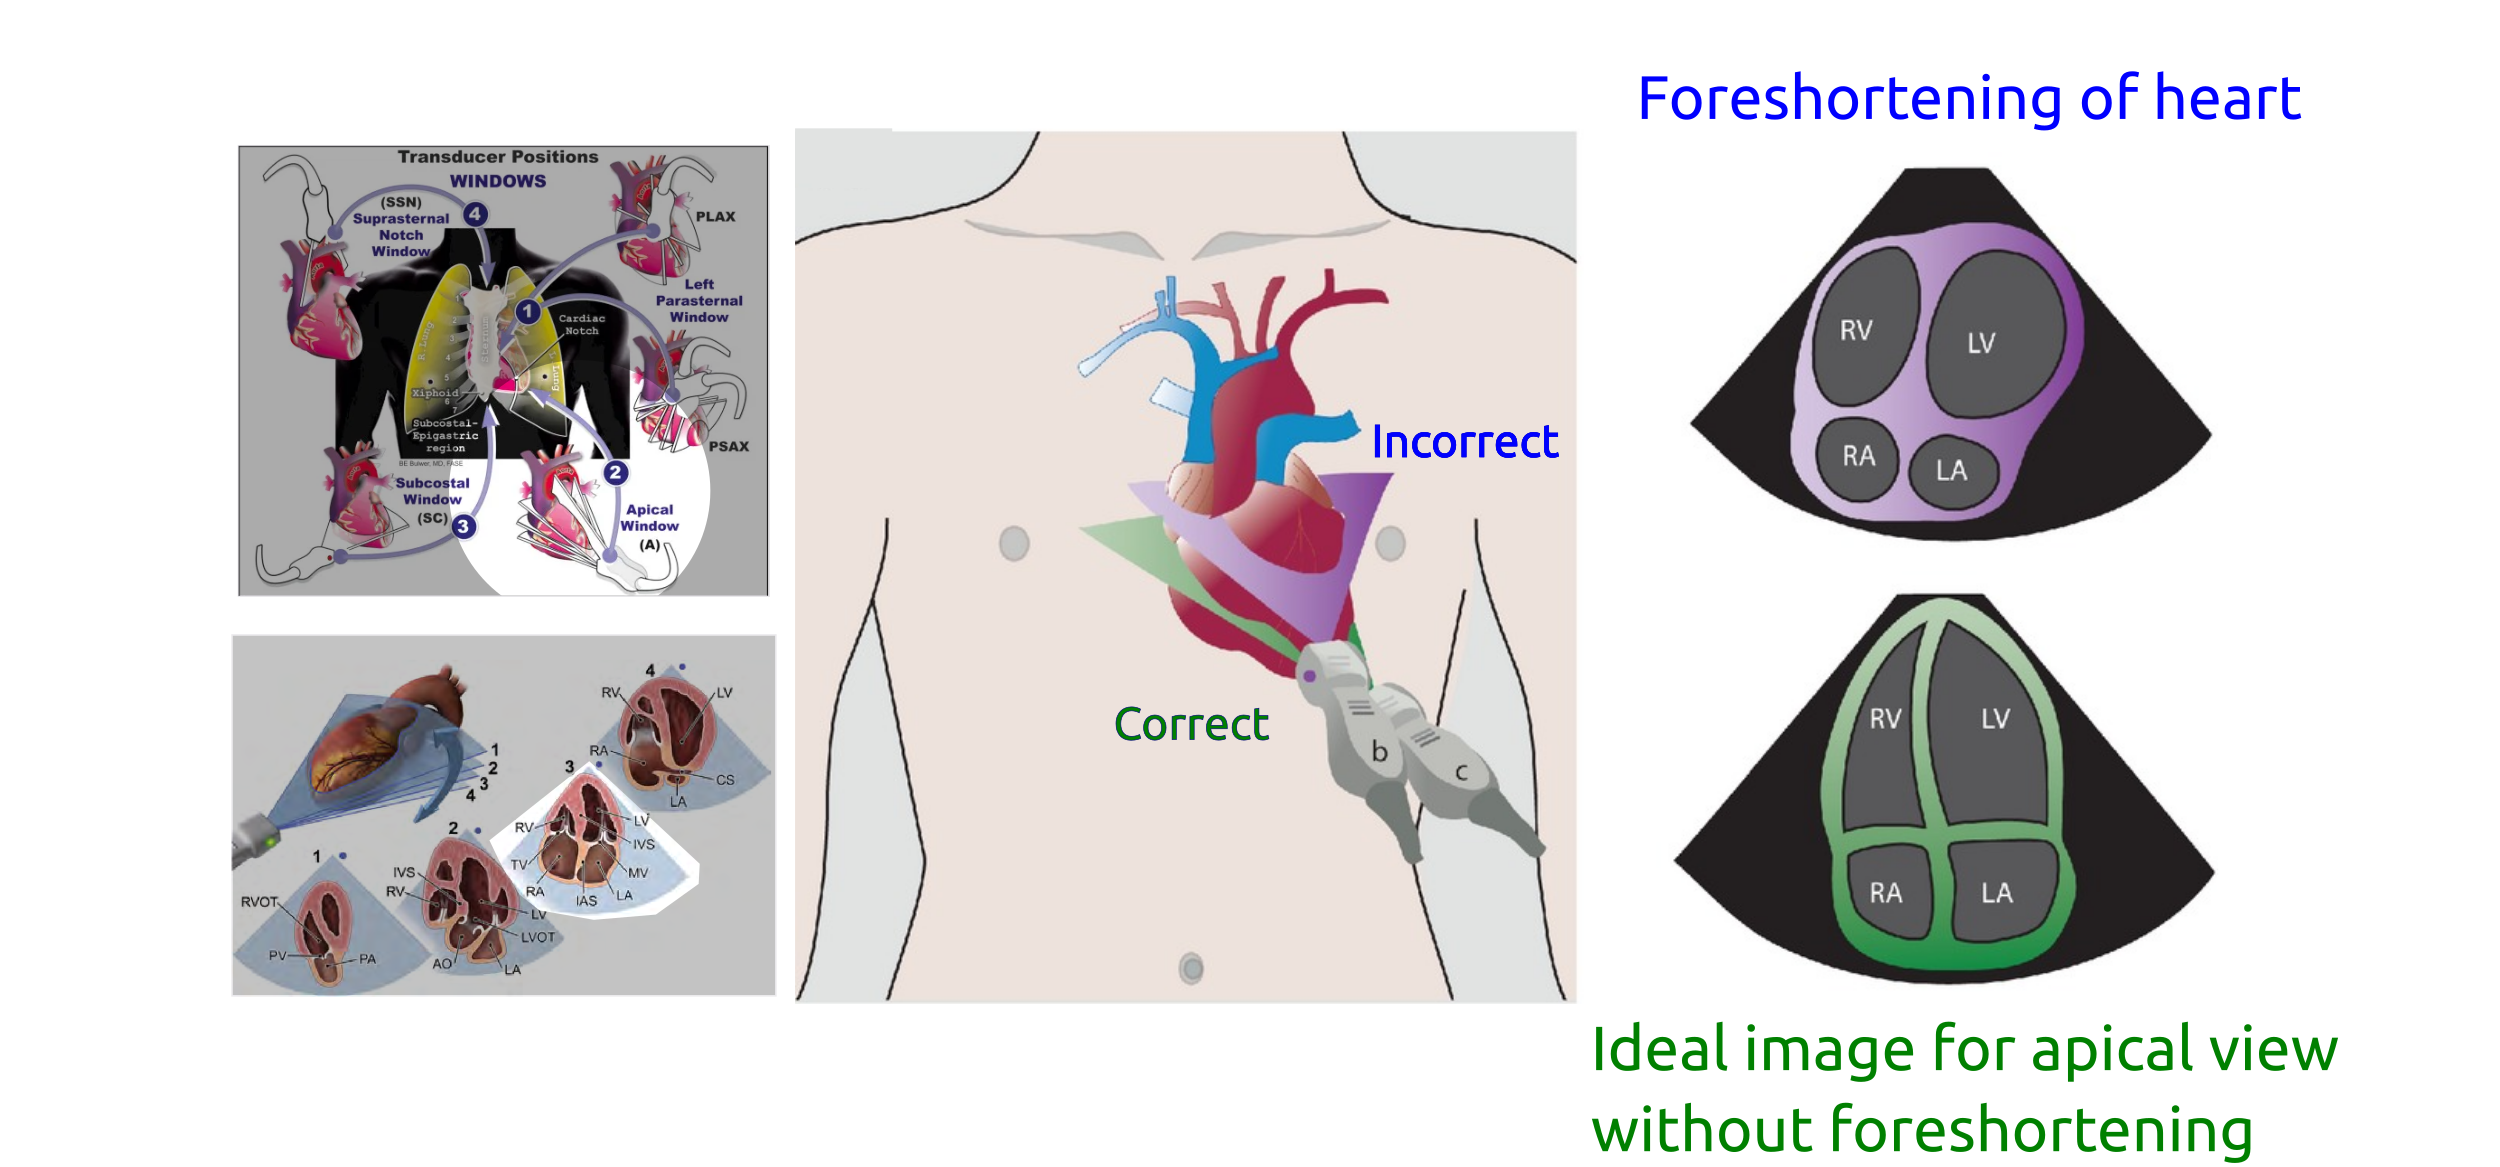
\includegraphics[width=1.0\textwidth]{ai-enable-echocardiography-A/versions/drawing-v00}
        % \caption{The sonographer-probe-patient control system}
      \end{figure}
\end{frame}
}


%%%%%%%%%%%%%%%%%%%%%%%%%%%%%%%%%%%%%%%%%%%%%%%%%%%%%%%%
{

\begin{frame}{Processing videos for echocardiography}
      \begin{figure}
        \centering
        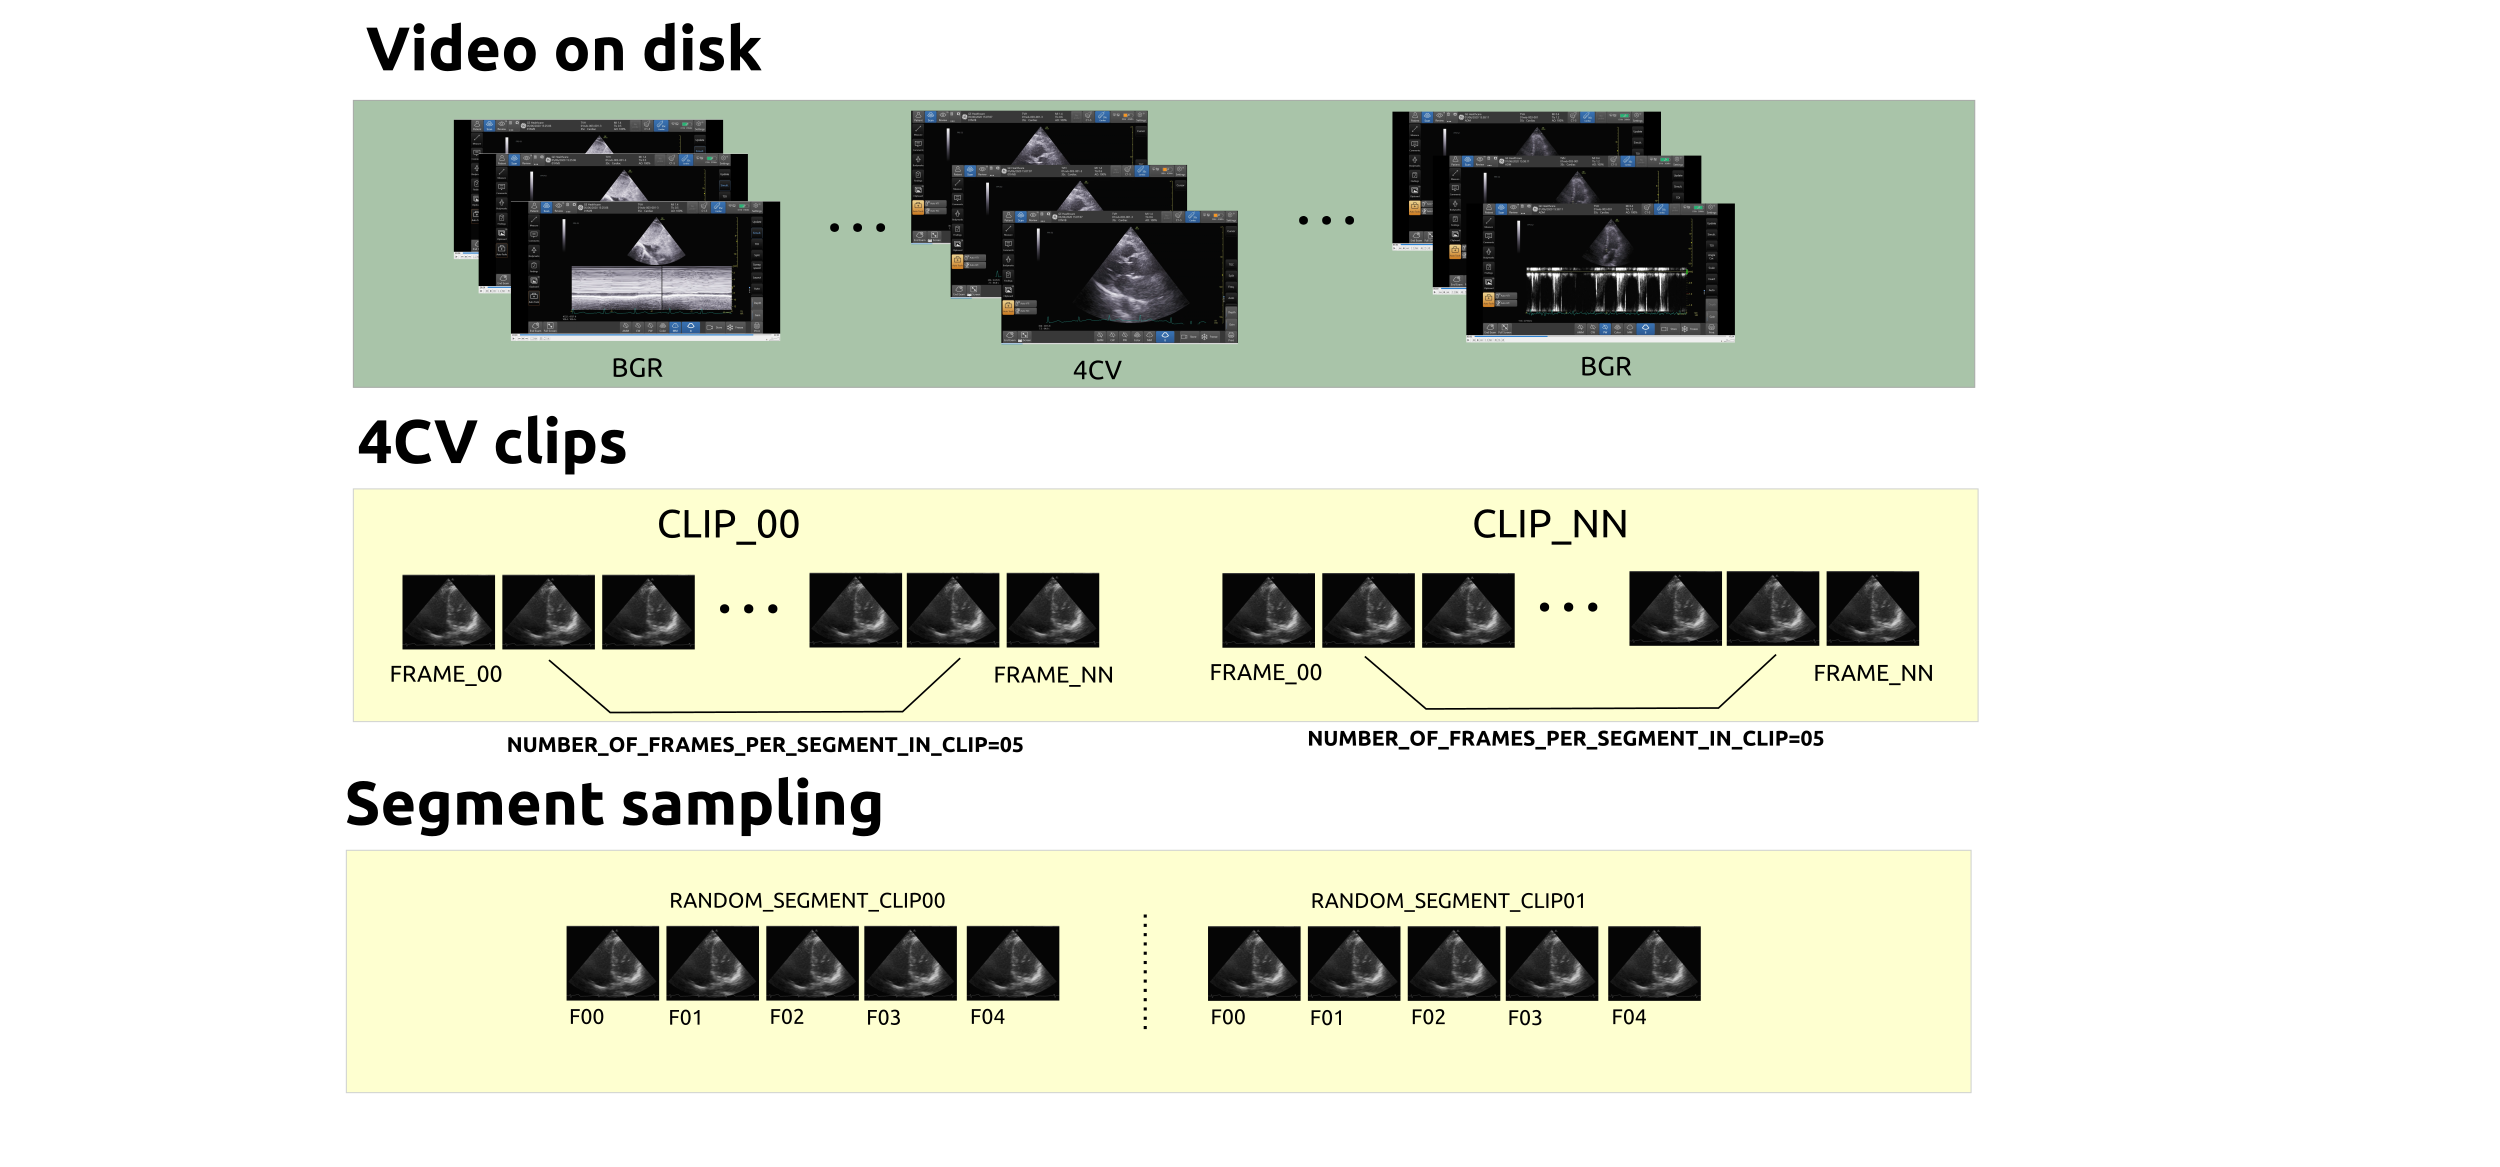
\includegraphics[width=1.0\textwidth]{ai-enable-echocardiography-B/versions/drawing-v00}
        % \caption{The sonographer-probe-patient control system}
      \end{figure}
\end{frame}
}


%%%%%%%%%%%%%%%%%%%%%%%%%%%%%%%%%%%%%%%%%%%%%%%%%%%%%%%%
{

\begin{frame}{Classification of US images with thinner neural networks}
      \begin{figure}
        \centering
        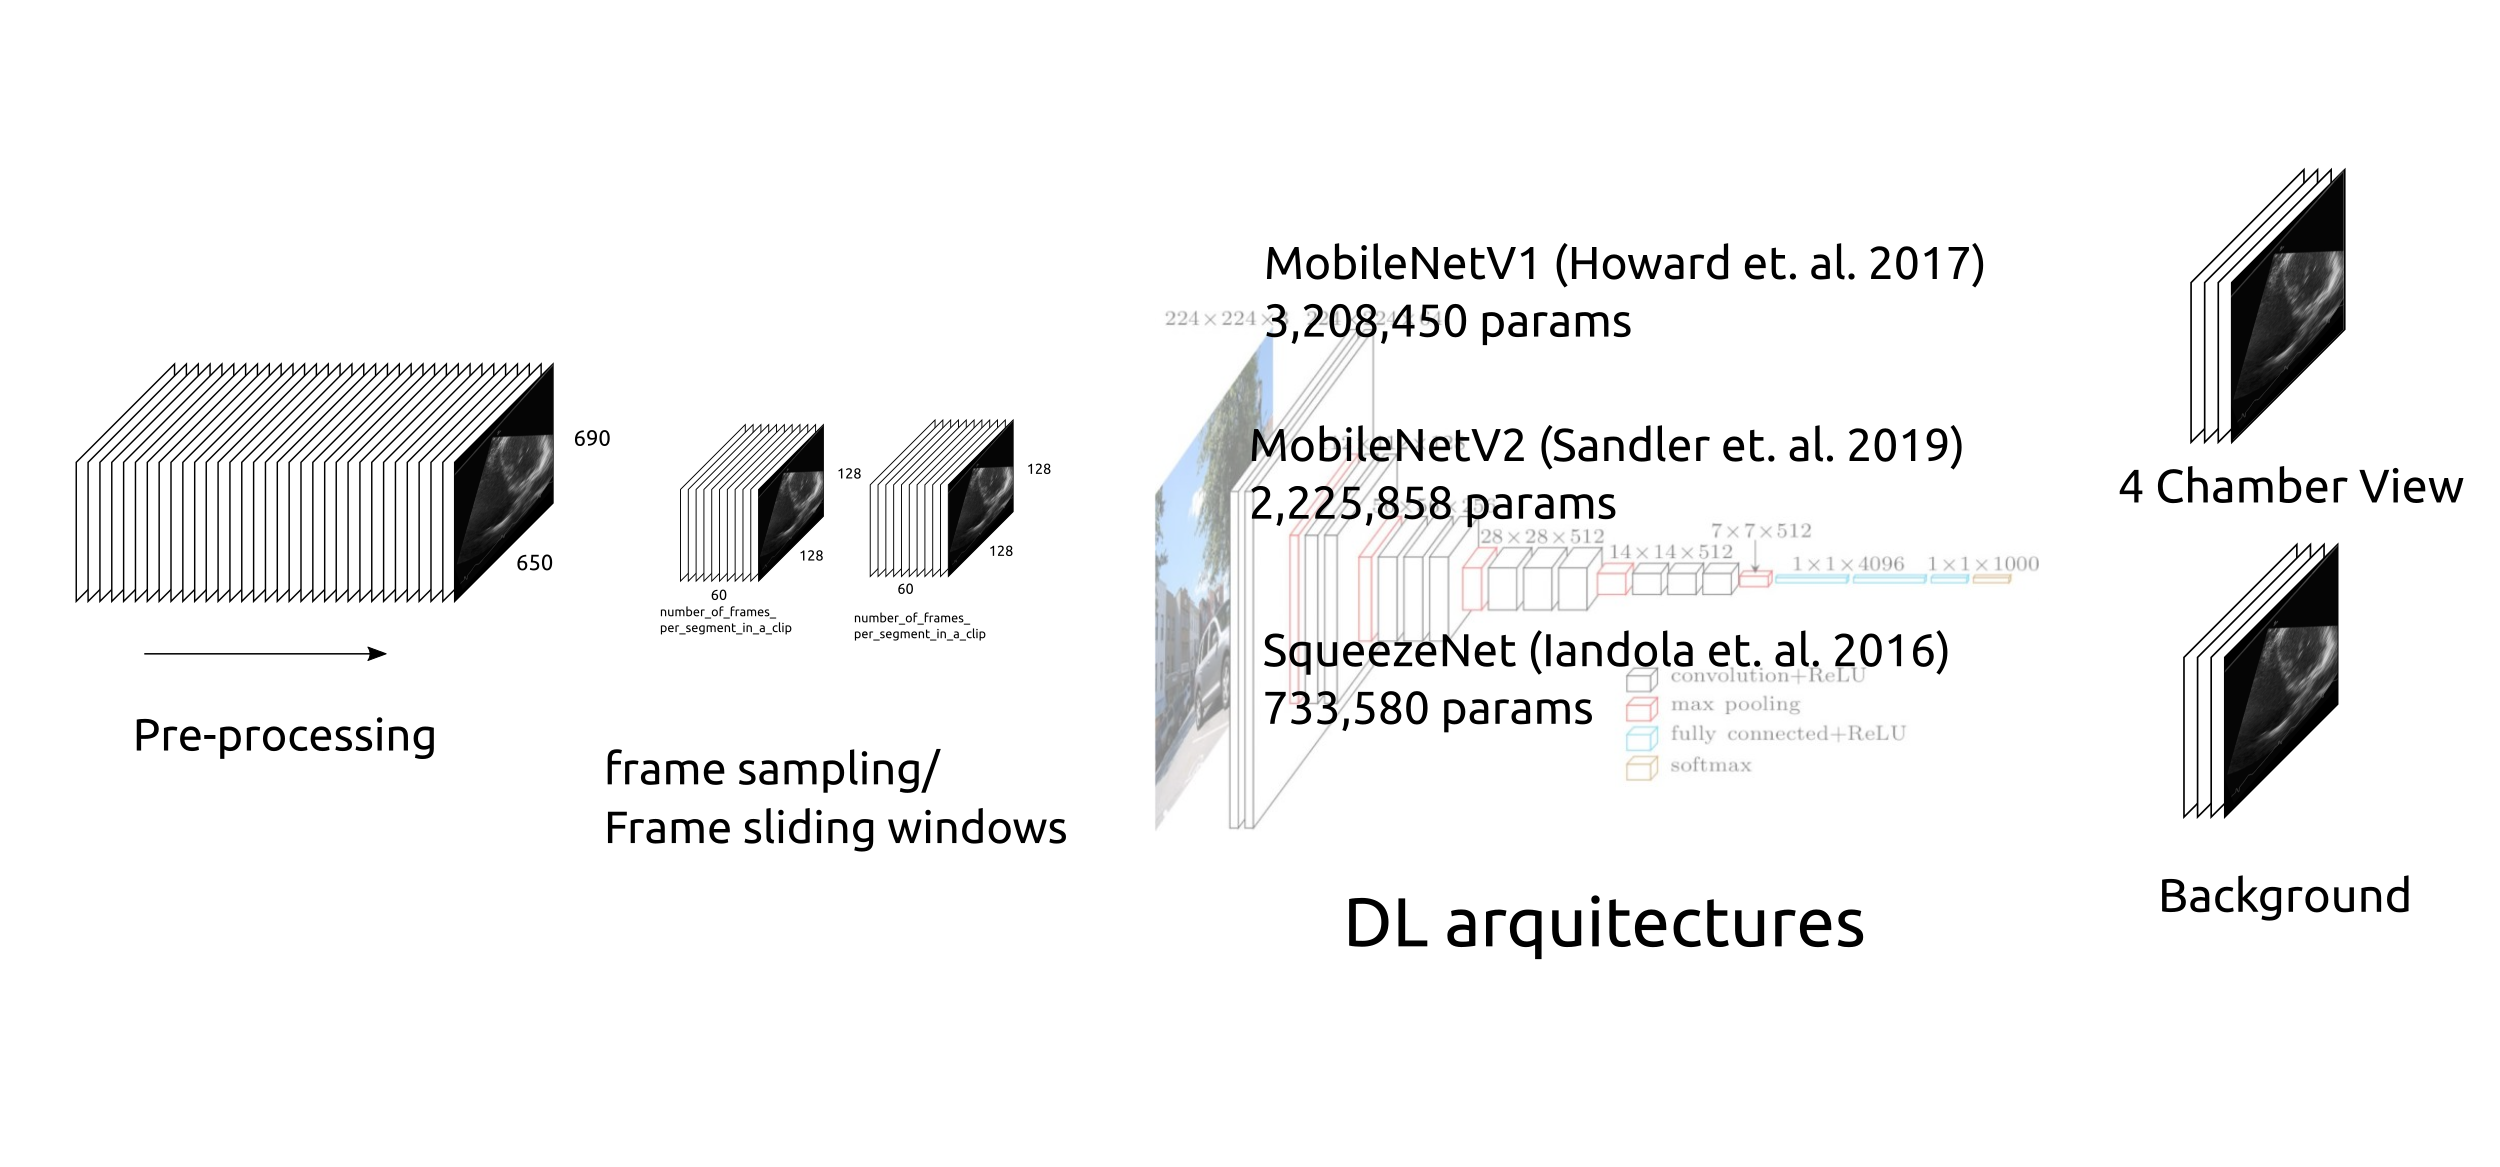
\includegraphics[width=1.0\textwidth]{ai-enable-echocardiography-C/versions/drawing-v00}
        % \caption{The sonographer-probe-patient control system}
      \end{figure}
\end{frame}
}

%%%%%%%%%%%%%%%%%%%%%%%%%%%%%%%%%%%%%%%%%%%%%%%%%%%%%%%%
{

\begin{frame}{Low-cost clinical system}
      \begin{figure}
        \centering
        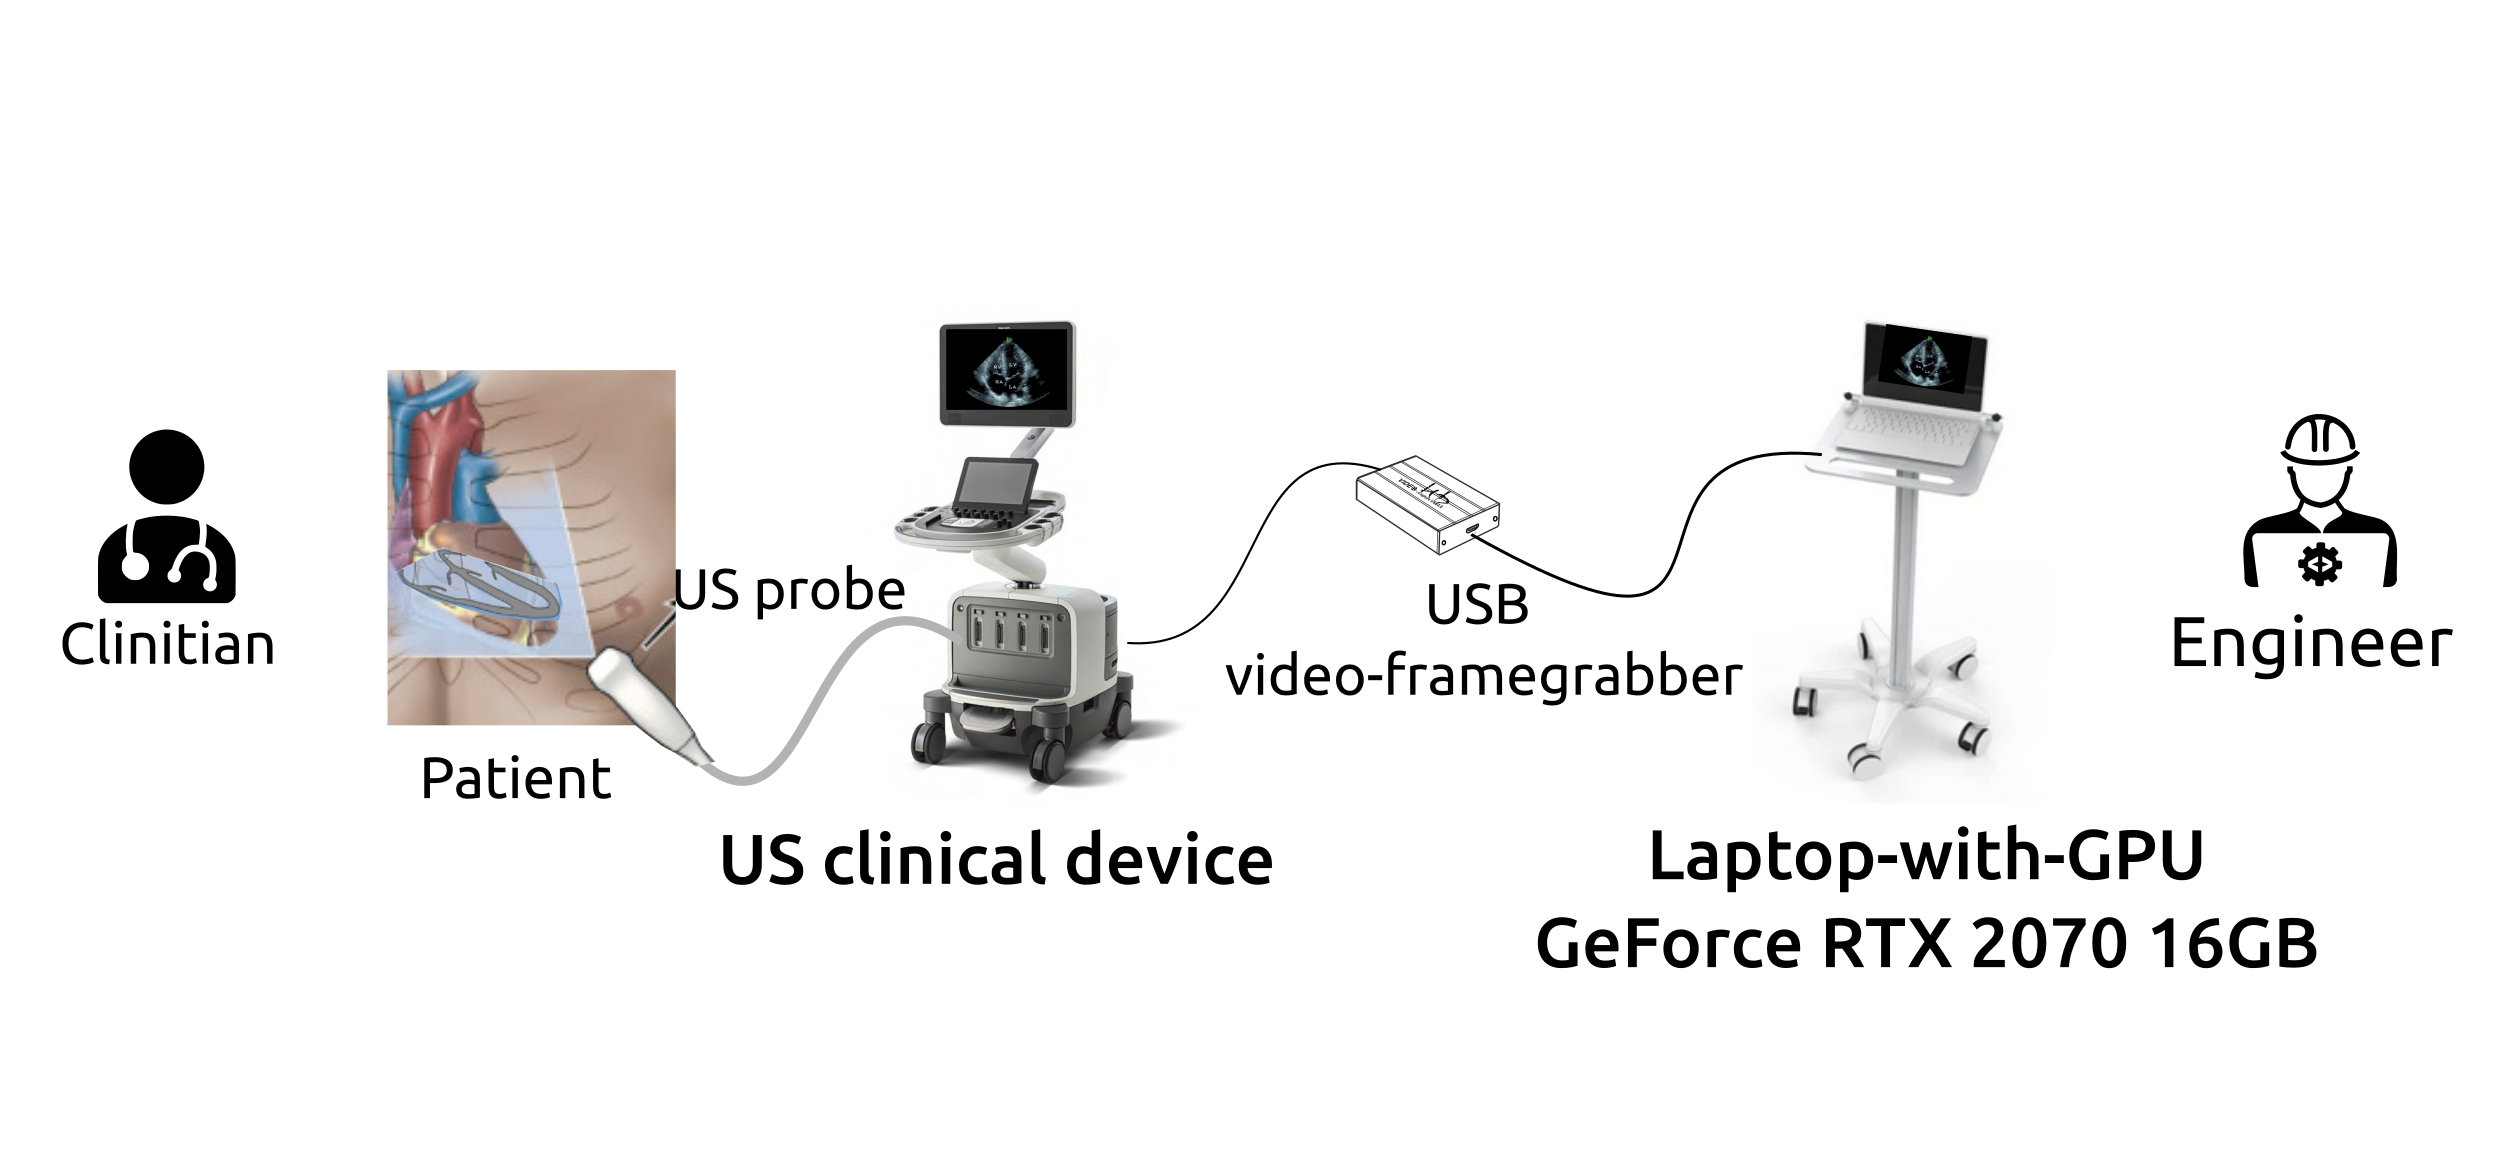
\includegraphics[width=1.0\textwidth]{ai-enable-echocardiography-D/versions/drawing-v00}
        % \caption{The sonographer-probe-patient control system}
      \end{figure}
\end{frame}
}





%%%%%%%%%%%%%%%%%%%%%%%%%%%%%%%%%%%%%%%%%%%%
\section{Ultrasound Image Synthesis}

\begin{frame}
  \frametitle{Table of Contents}
  \tableofcontents[currentsection]
\end{frame}




\subsection{Clinical background}

%%%%%%%%%%%%%%%%%%%%%%%%%%%%%%%%%%%%%%%%%%%%%%%%%%%%%%%%
{
\paper{
Wright-Gilbertson M. 2014 in PhD thesis; \url{https://en.wikipedia.org/wiki/Gestational_age}; 
National-Health-Service 2021. Screening for down’s syndrome, edwards’ syndrome and patau’s syndrome. \url{https://www.nhs.uk/pregnancy/your-pregnancy-care} 
}

\begin{frame}{Dating US scan (12-week scan)}
      \begin{figure}
        \centering
        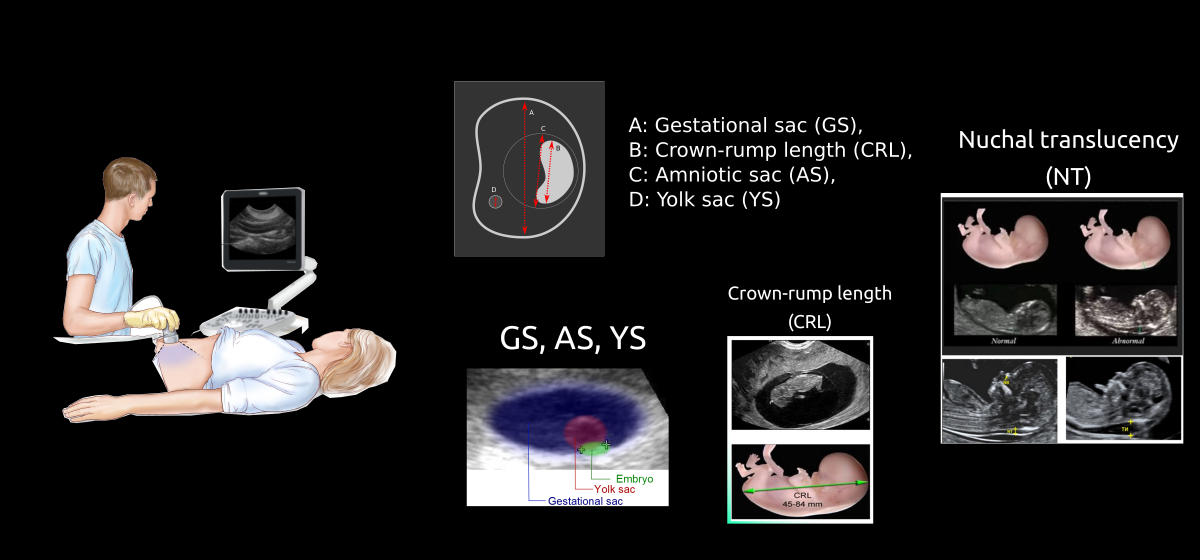
\includegraphics[width=1.0\textwidth]{12-week-scan/versions/drawing-v01}
        % \caption{The sonographer-probe-patient control system}
      \end{figure}
\end{frame}
}



%%%%%%%%%%%%%%%%%%%%%%%%%%%%%%%%%%%%%%%%%%%%%%%%%%%%%%%%
{
\paper{
Sciortino et al. in Computers in Biology and Medicine 2017 https://doi.org/10.1016/j.compbiomed.2017.01.008; 
He et al. in Front. Med. 2021 https://doi.org/10.3389/fmed.2021.729978
}
\begin{frame}{Challenges of ultrasound biometric measurements}	

\begin{itemize}
\item Operator dependant 
\item Position of the baby
\item Similar morphological and echogenic characteristics in the US
% \item Threshold selection of the binary masks 
\item Few public datasets are available (we have only found two)
%https://www.nature.com/articles/jhg200888
\end{itemize}

\end{frame}
}




\subsection{Research aims}


%%%%%%%%%%%%%%%%%%%%%%%%%%%%%%%%%%%%%%%%%%%%%%%%%%%%%%%%
{
%\paper{Wright-Gilbertson M. 2014 in PhD thesis}
\begin{frame}{Research aims}	
\begin{itemize}
\item Investigate and implement deep-learning methods for synthetic fetal ultrasound imaging of normal and abnormal cases;
\item Propose and apply methods to evaluate quantitative and qualitative images to investigate fetal biomechanics; and 
\item Design and  test fetal phantoms that mimic various poses, and fetal ages.
% \item 
\end{itemize}

\end{frame}
}



%%%%%%%%%%%%%%%%%%%%%%%%%%%%%%%%%%%%%%%%%%%%%%%%%%%%%%%%
{
% \paper{Private github repository: \url{https://github.com/xfetus/synthetic-foetuses​}}
\begin{frame}{GAN-based fetal US imaging}
      \begin{figure}
        \centering
        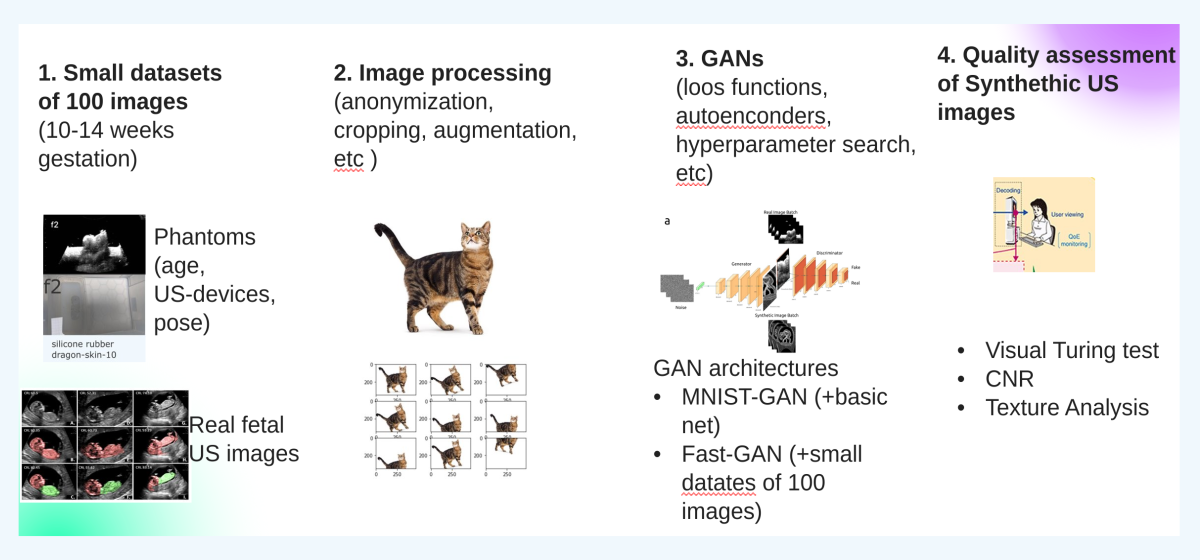
\includegraphics[width=1.0\textwidth]{gans-based-pipeline-fetal-imaging-pipeline/versions/drawing-v00}
        %\caption{}
      \end{figure}
\end{frame}
}

%%%%%%%%%%%%%%%%%%%%%%%%%%%%%%%%%%%%%%%%%%%%%%%%%%%%%%%%
{
\paper{(a) Bautista et al. 2022, "Empirical Study of Quality Image Assessment for Synthesis of Fetal Head Ultrasound Imaging with DCGANs" MIUA https://github.com/budai4medtech/miua2022 (b) Liu et al. 2021 "Towards Faster and Stabilized GAN Training for High-fidelity Few-shot Image Synthesis" https://arxiv.org/abs/2101.04775 }

\begin{frame}{GAN-based fetal imaging}
      \begin{figure}
        \centering
        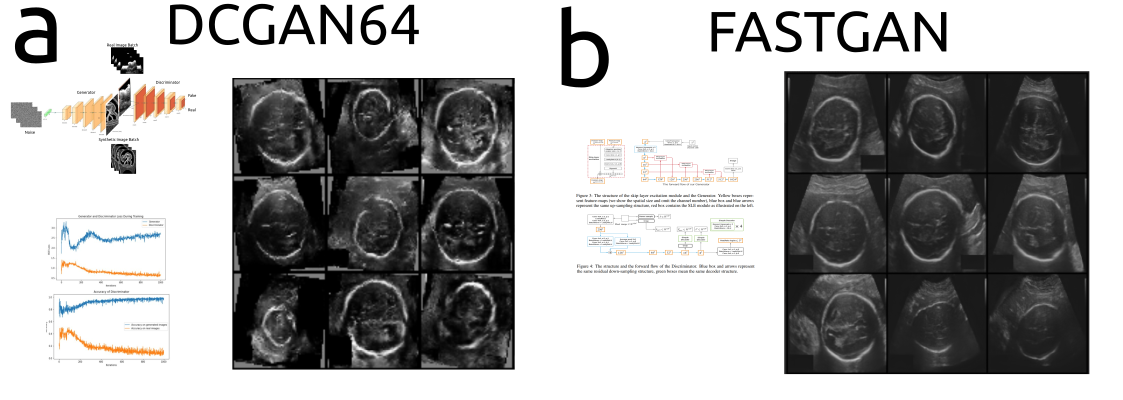
\includegraphics[width=1.0\textwidth]{gan-based-fetal-imaging/versions/drawing-v01}
        \caption{(a) DCGAN arquitecture, loss functions for DC-GANs and batches of synthetic fetal head images,
		(b) FASTGAN arquitecture and batches of synthethic fetal head images}
      \end{figure}
\end{frame}
}

%%%%%%%%%%%%%%%%%%%%%%%%%%%%%%%%%%%%%%%%%%%%%%%%%%%%%%%%
{
\paper{
(a) Ho et al. 2020 "Denoising Diffusion Probabilistic Models" https://arxiv.org/abs/2006.11239 
(b) Fiorentino et al. 2022 "A Review on Deep-Learning Algorithms for Fetal Ultrasound-Image Analysis" https://arxiv.org/abs/2201.12260
}

\begin{frame}{Difussion models for fetal imaging}
      \begin{figure}
        \centering
        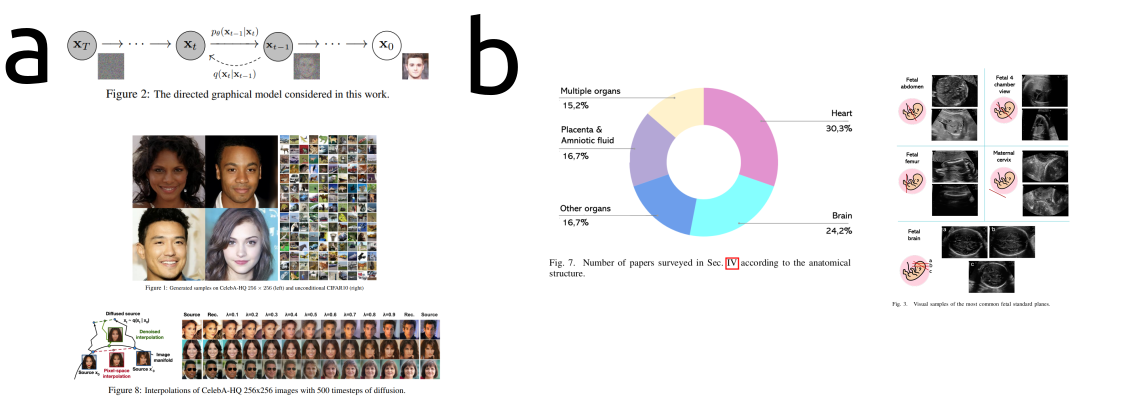
\includegraphics[width=1.0\textwidth]{diffusion-based-generative-models/versions/drawing-v00}
        %\caption{(a) DCGAN arquitecture, loss functions for DC-GANs and batches of synthetic fetal head images,
	%	(b) FASTGAN arquitecture and batches of synthethic fetal head images}
      \end{figure}
\end{frame}
}


\subsection{Phantoms for AI-based fetal biomechanics}

%%%%%%%%%%%%%%%%%%%%%%%%%%%%%%%%%%%%%%%%%%%%%%%%%%%%%%%%
{
% \paper{Private github repository: \url{https://github.com/xfetus/synthetic-foetuses​}}
\begin{frame}{Phantoms for AI-based fetal biomechanics}
      \begin{figure}
        \centering
        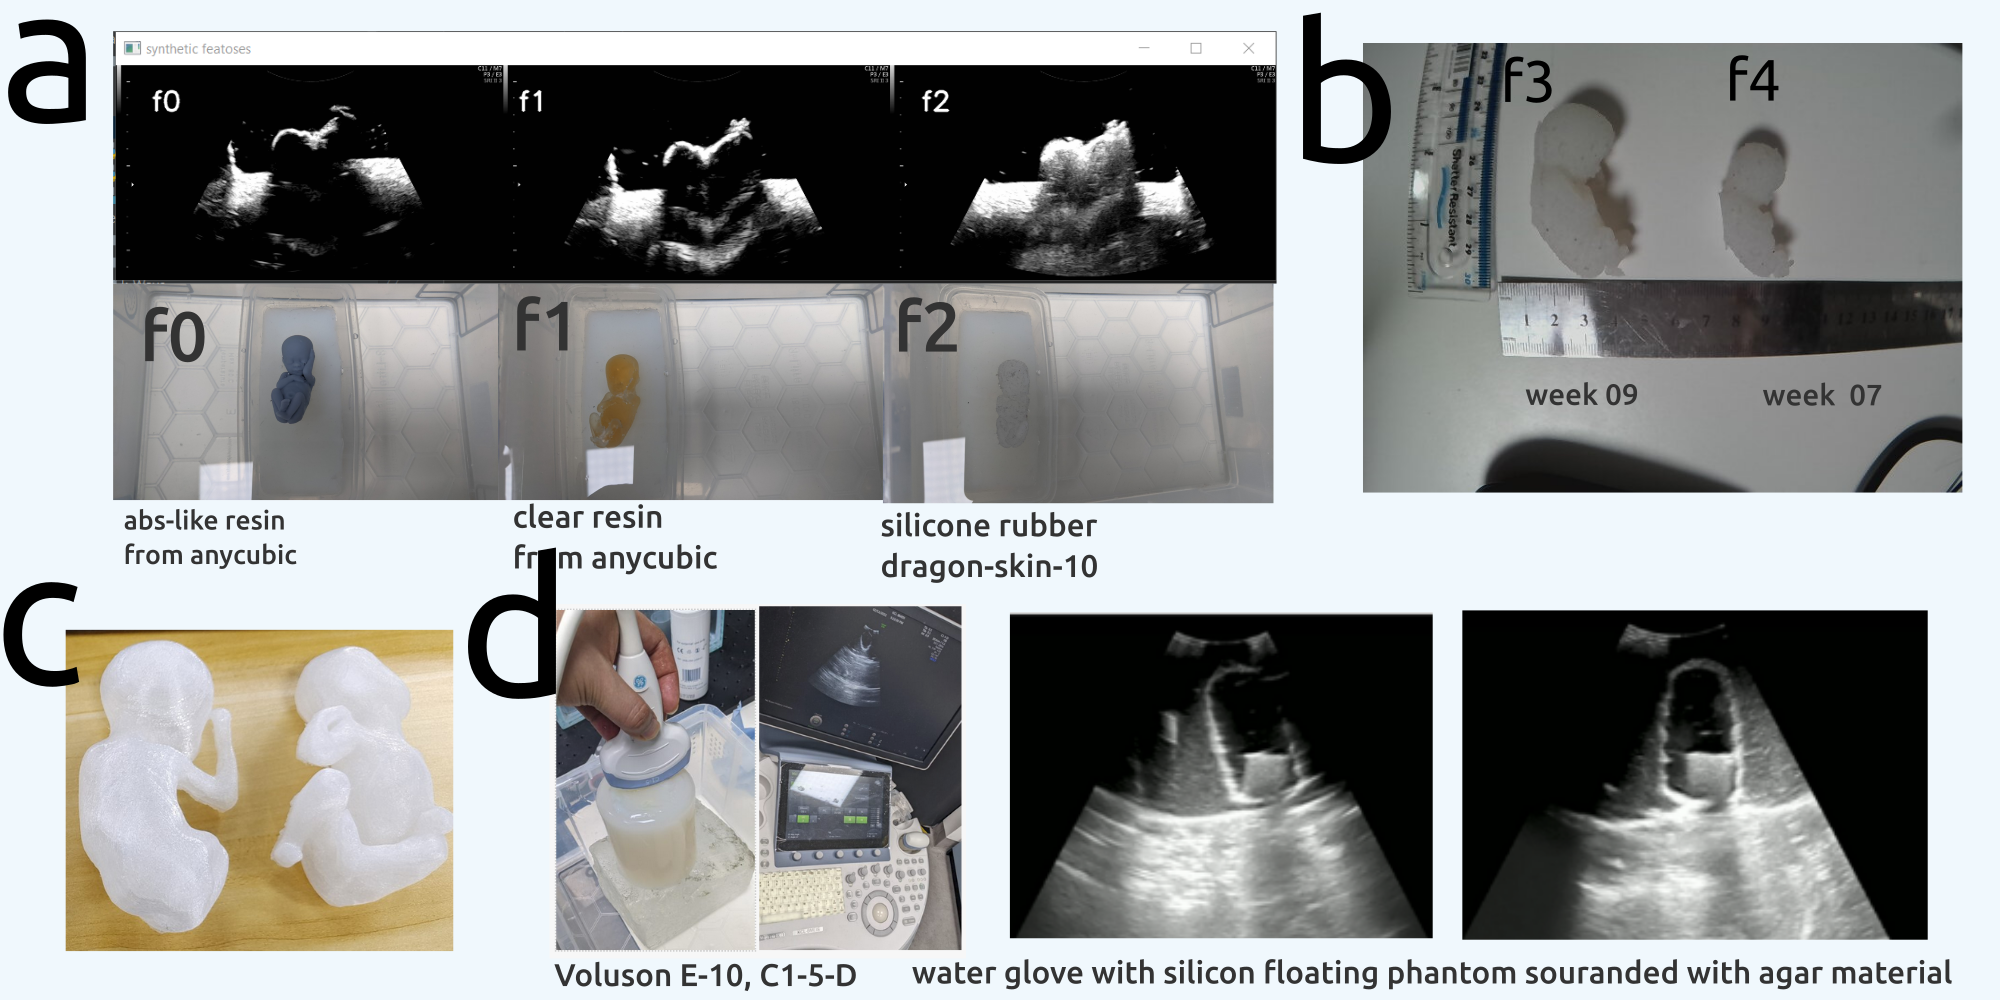
\includegraphics[width=1.0\textwidth]{us-images-of-3d-printed-fetuses/versions/drawing-v05}
        %\caption{}
      \end{figure}
\end{frame}
}




%%%%%%%%%%%%%%%%%%%%%%%%%%%%%%%%%%%%%%%%%%%%
\subsection{Building AI for Medical Devices}


%%%%%%%%%%%%%%%%%%%%%%%%%%%%%%%%%%%%%%%%%%%%%%%%%%%%%%%%
{
%\paper{(a) Coordinate systems overview sketch in 3D Slicer,  (b) Asselin et al. 2018 in conf-BIVPCS, (c) US-simulator, and (d) 3D-printed fetus}
\paper{
Clara AGX: https://www.nvidia.com/en-gb/clara/intelligent-medical-instruments/;
Clara holoscan EGX: https://developer.nvidia.com/clara-holoscan-sdk
}
\begin{frame}{Building AI for Medical Devices}

      \begin{figure}
        \centering
        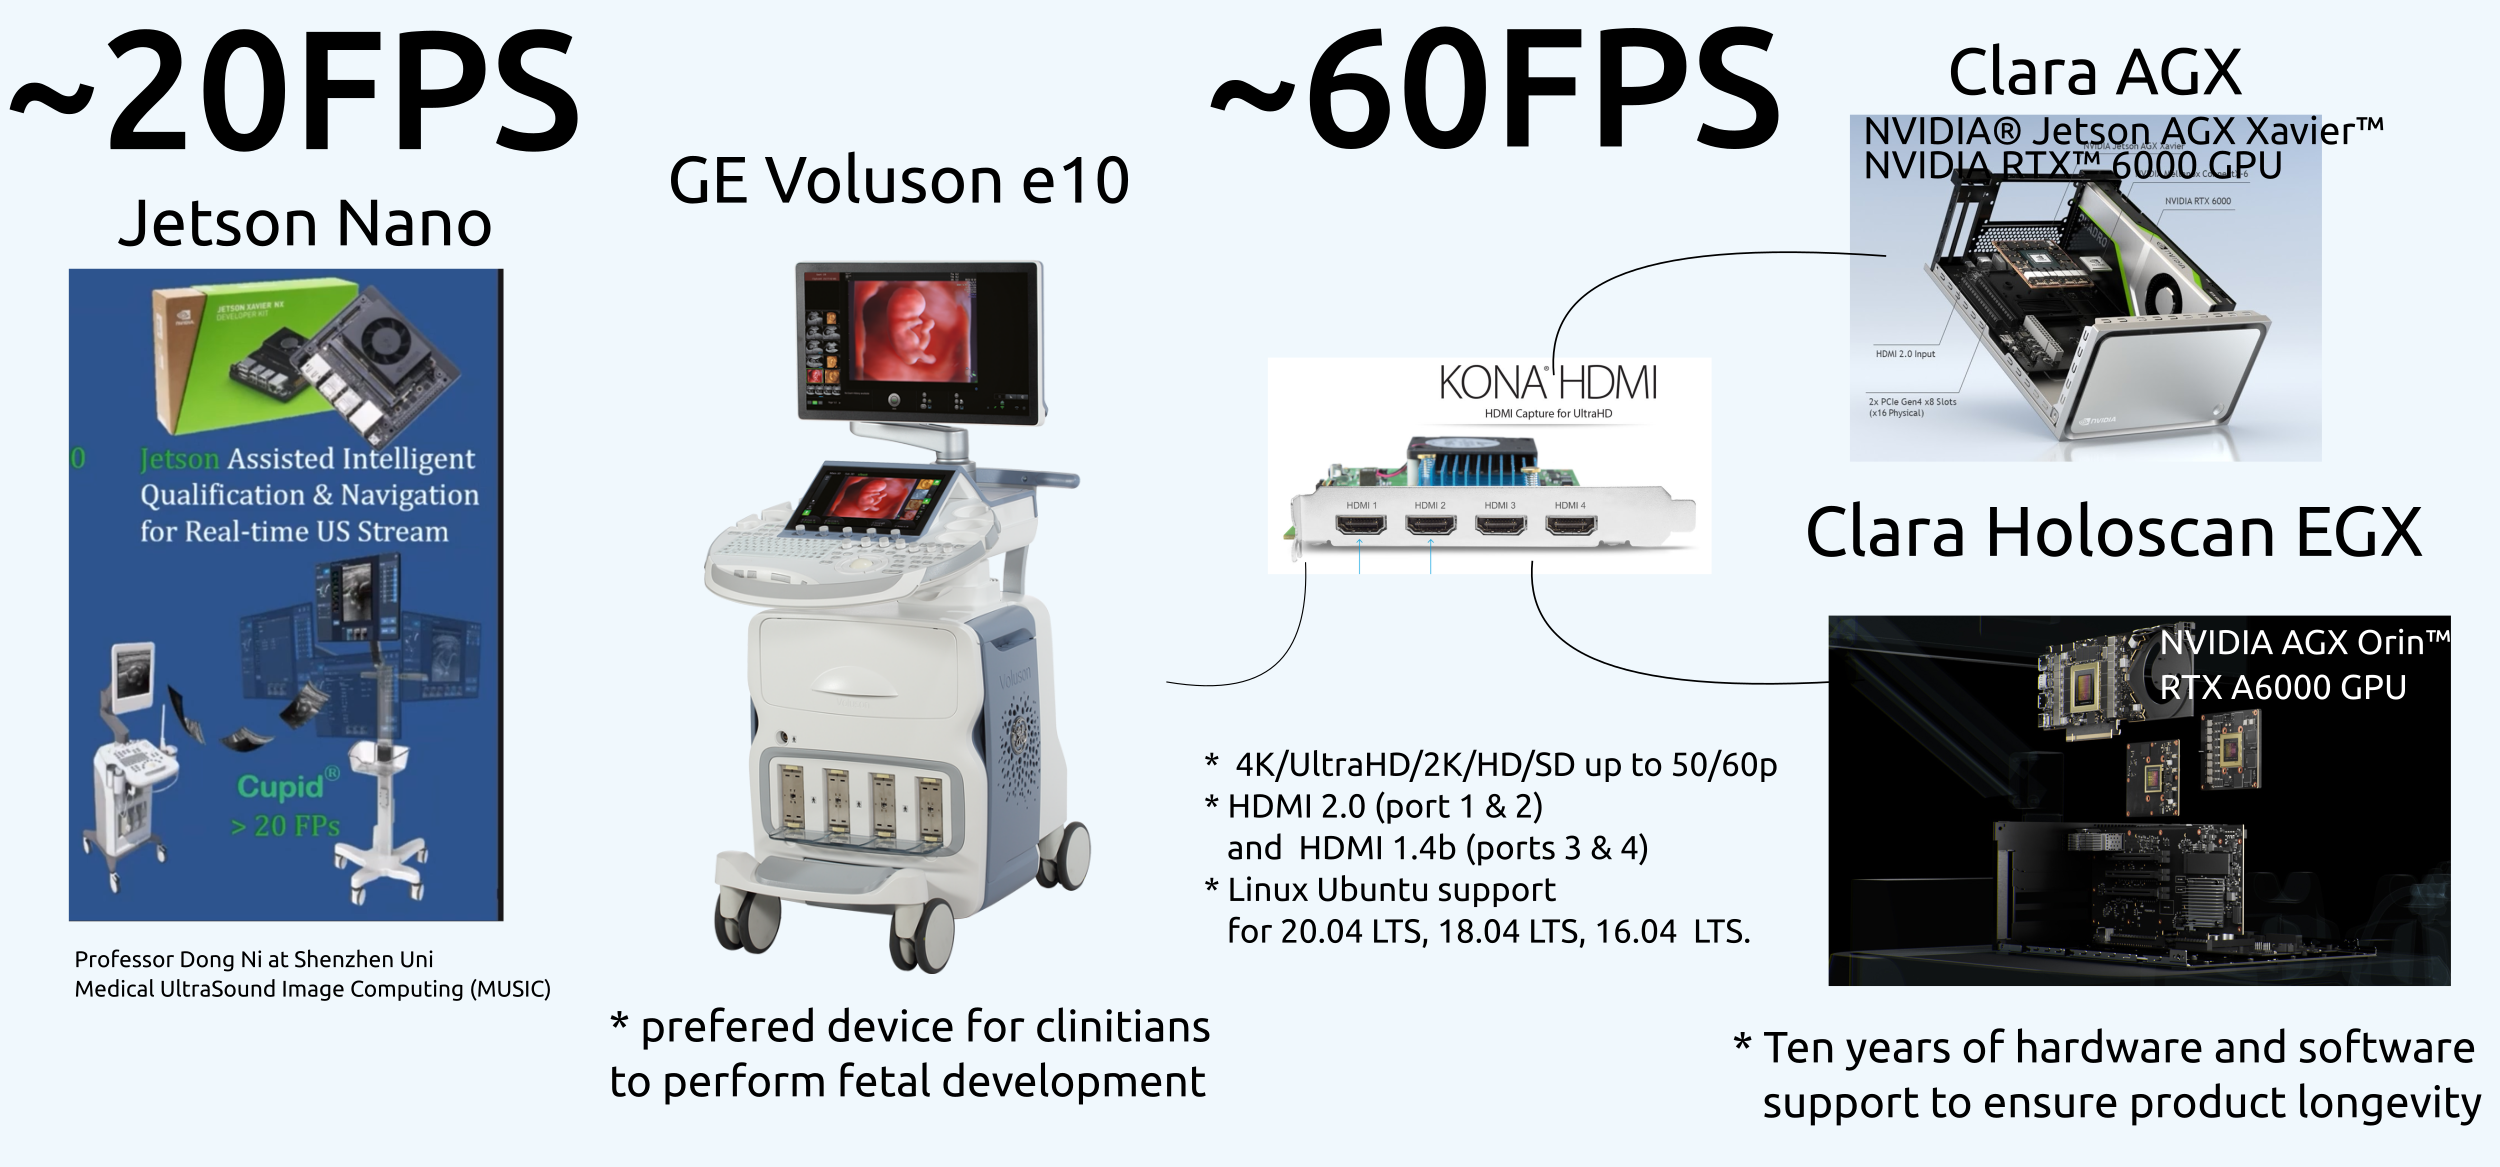
\includegraphics[width=1.0\textwidth]{medical-devices/versions/drawing-v01}
      \end{figure}


\end{frame}
}



% %%%%%%%%%%%%%%%%%%%%%%%%%%%%%%%%%%%%%%%%%%%%
% \subsection{Potential outcomes}

% %%%%%%%%%%%%%%%%%%%%%%%%%%%%%%%%%%%%%%%%%%%%%%%%%%%%%%%%
% {
% %\paper{(a) Coordinate systems overview sketch in 3D Slicer,  (b) Asselin et al. 2018 in conf-BIVPCS, (c) US-simulator, and (d) 3D-printed fetus}
% %\paper{}
% \begin{frame}{Potential outcomes}


%       \begin{figure}
%         \centering
%         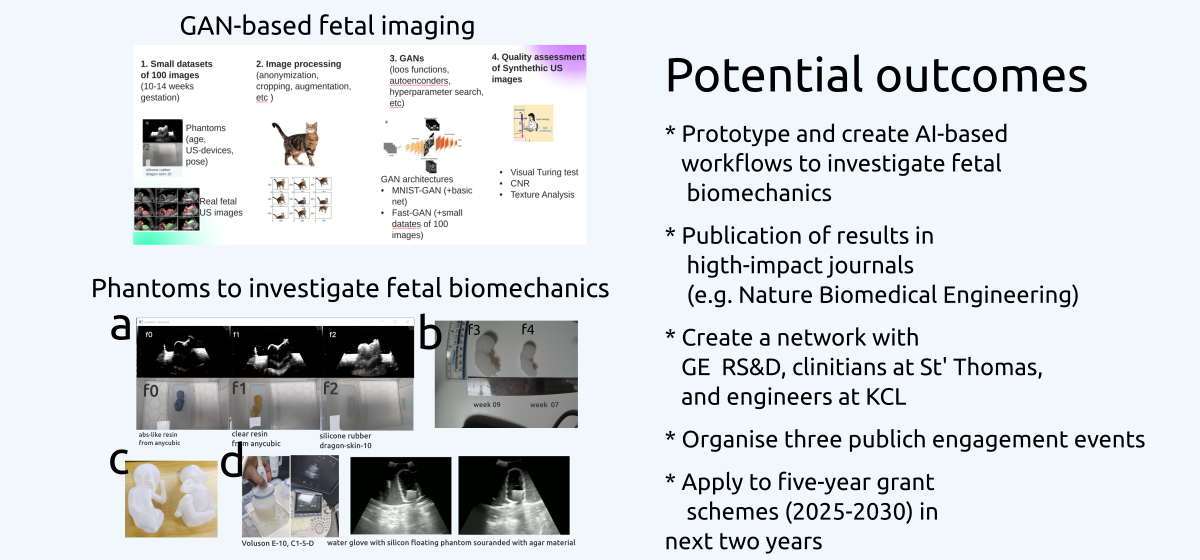
\includegraphics[width=1.0\textwidth]{potential-outcomes/versions/drawing-v00.png}
%       \end{figure}


% \end{frame}
% }





% %%%%%%%%%%%%%%%%%%%%%%%%%%%%%%%%%%%%%%%%%%%%%%%%%%%%%%%%
% {
% %\paper{Wright-Gilbertson M. 2014 in PhD thesis}
% \begin{frame}{Research Questions}	
%  %Can we understand more about fetal development trough the development of more realistic phantoms
% %Can dynamic fetal phantoms be created to understand fetal development?  %added Thu 15 Apr 05:20:09 BST 2021
% %Can synthetic fetus help to understand fetal development? %Fri 23 Apr 05:56:53 BST 2021
% %* Can the creation of synthetic fetuses help to understand fetal development? %Wed 12 May 08:20:58 BST 2021 
% %* Can the creation of synthetic fetuses predict fetal development issues? %Wed 12 May 09:50:47 BST 2021

% \BigSizeFont
% \begin{itemize}
% %\item Would the creation of synthetic fetuses help to understand 
% %the biomechatincs of phetal development? %Sat 15 May 14:51:42 BST 2021
% %\item Can we understand fetal development with synthetic fetuses? %Sat 15 May 15:08:19 BST 2021
% %\item Can the understanding of fetal biomechanics lead to predict fetal pathologies? %Mon 12 Jul 09:25:41 BST 2021
% % MORE ON FETAL PATHOLOGIES:https://www.sciencedirect.com/topics/medicine-and-dentistry/fetal-pathology
% \item Can fetal biomechanics help to understand the prediction of fetal pathologies? %% Mon 12/07/2021 09:45
% \item Would AI-based fetal biomechanics automatically predict fetal pathologies? %Tue 19 Oct 16:54:45 BST 2021
% \item \end{itemize}

% \end{frame}
% }



% %%%%%%%%%%%%%%%%%%%%%%%%%%%%%%%%%%%%%%%%%%%%%%%%%%%%%%%%
% {
% %\paper{Wright-Gilbertson M. 2014 in PhD thesis}
% \begin{frame}{Research Questions}	
%  %Can we understand more about fetal development trough the development of more realistic phantoms
% %Can dynamic fetal phantoms be created to understand fetal development?  %added Thu 15 Apr 05:20:09 BST 2021
% %Can synthetic fetus help to understand fetal development? %Fri 23 Apr 05:56:53 BST 2021
% %* Can the creation of synthetic fetuses help to understand fetal development? %Wed 12 May 08:20:58 BST 2021 
% %* Can the creation of synthetic fetuses predict fetal development issues? %Wed 12 May 09:50:47 BST 2021

% \BigSizeFont
% \begin{itemize}
% %\item Would the creation of synthetic fetuses help to understand 
% %the biomechatincs of phetal development? %Sat 15 May 14:51:42 BST 2021
% %\item Can we understand fetal development with synthetic fetuses? %Sat 15 May 15:08:19 BST 2021
% %\item Can the understanding of fetal biomechanics lead to predict fetal pathologies? %Mon 12 Jul 09:25:41 BST 2021
% % MORE ON FETAL PATHOLOGIES:https://www.sciencedirect.com/topics/medicine-and-dentistry/fetal-pathology
% % \item Can fetal biomechanics help to understand the prediction of fetal pathologies? %% Mon 12/07/2021 09:45
% % \item Would AI-based fetal biomechanics automatically predict fetal pathologies? %Tue 19 Oct 16:54:45 BST 2021

% \item Can GAN-based approaches help to address the scarcity of non-available datasets?
% \item How can AI-based algorthims be less user-dependant and machine-dependant?
% \end{itemize}

% \end{frame}
% }





%%%%%%%%%%%%%%%%%%%%%%%%%%%%%%%%%%%%%%%%%%%%
\section{Appendix}

\begin{frame}
  \frametitle{Table of Contents}
  \tableofcontents[currentsection]
\end{frame}


\subsection{I: Fetal Poses, II: Fetal Behaviours}

%%%%%%%%%%%%%%%%%%%%%%%%%%%%%%%%%%%%%%%%%%%%%%%%%%%%%%%%
{
\paper{Ferguson and Haultain 1889 in Handbook of Obstetric Nursing, pages 150–153; Mori et al. 2010 in ICDL}
\begin{frame}{I: Fetal Poses, II: Fetal Behaviours}
      \begin{figure}
        \centering
        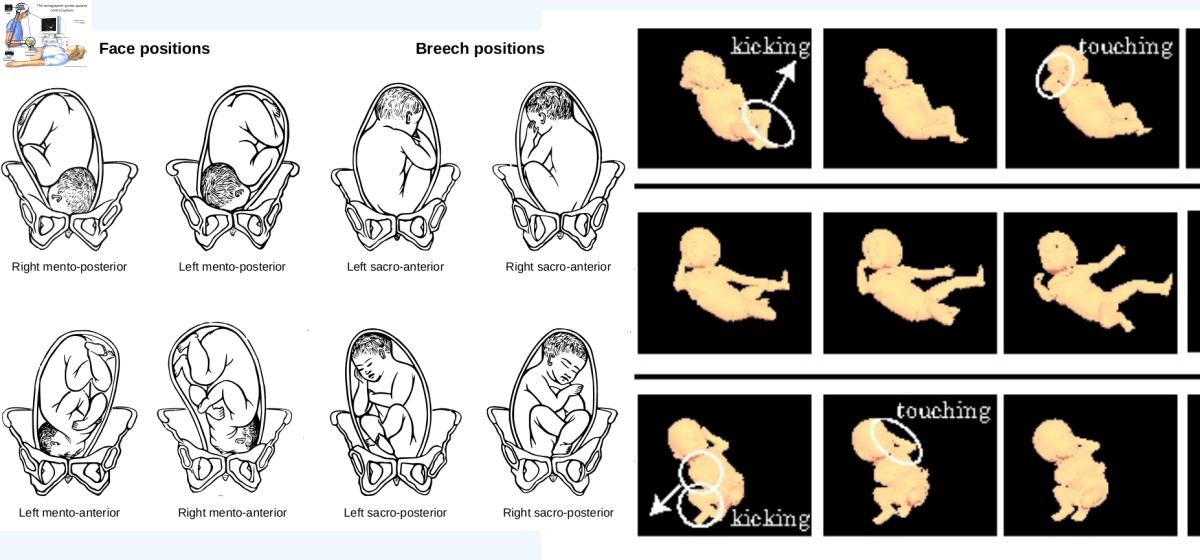
\includegraphics[width=1.0\textwidth]{fetal-poses/versions/drawing-v01.png}
        %\caption{}
      \end{figure}
\end{frame}
}

\subsection{Growing Baby: 3D Print-ready Models}


%%%%%%%%%%%%%%%%%%%%%%%%%%%%%%%%%%%%%%%%%%%%%%%%%%%%%%%%
{
\paper{Growing Baby: 3D Print-ready Models}
\begin{frame}{III: Fetal Growth}
      \begin{figure}
        \centering
        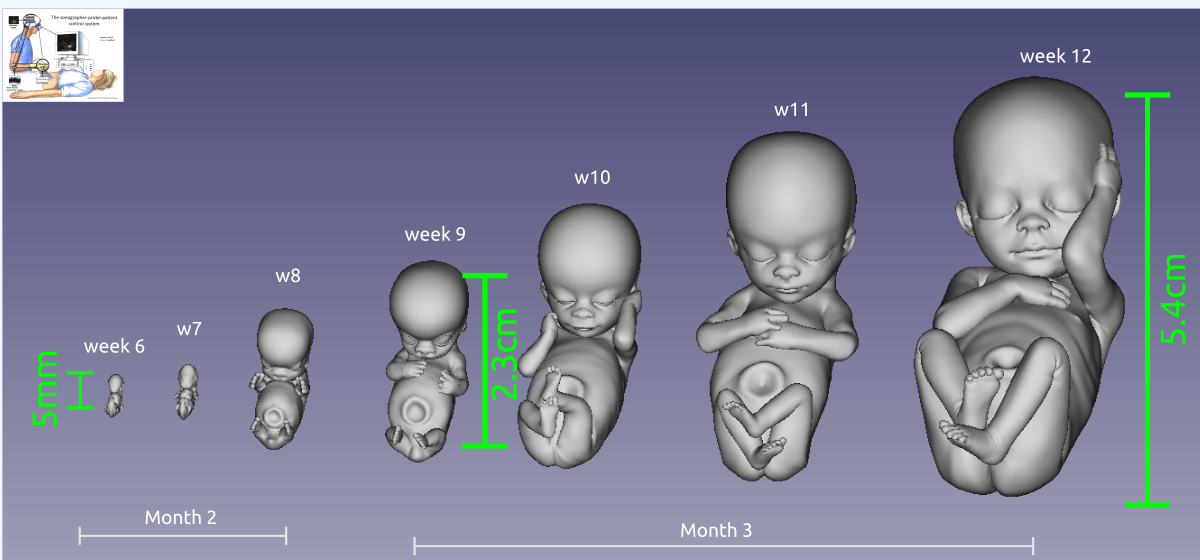
\includegraphics[width=1.0\textwidth]{fetal-ages/versions/drawing-v02.png}
        %\caption{}
      \end{figure}
\end{frame}
}


\subsection{State-of-the-art on modelling fetus}

%%%%%%%%%%%%%%%%%%%%%%%%%%%%%%%%%%%%%%%%%%%%%%%%%%%%%%%%
{
%\paper{Wright-Gilbertson M. 2014 in PhD thesis}
\begin{frame}{State-of-the-art on modelling fetus}
      \begin{figure}
        \centering
        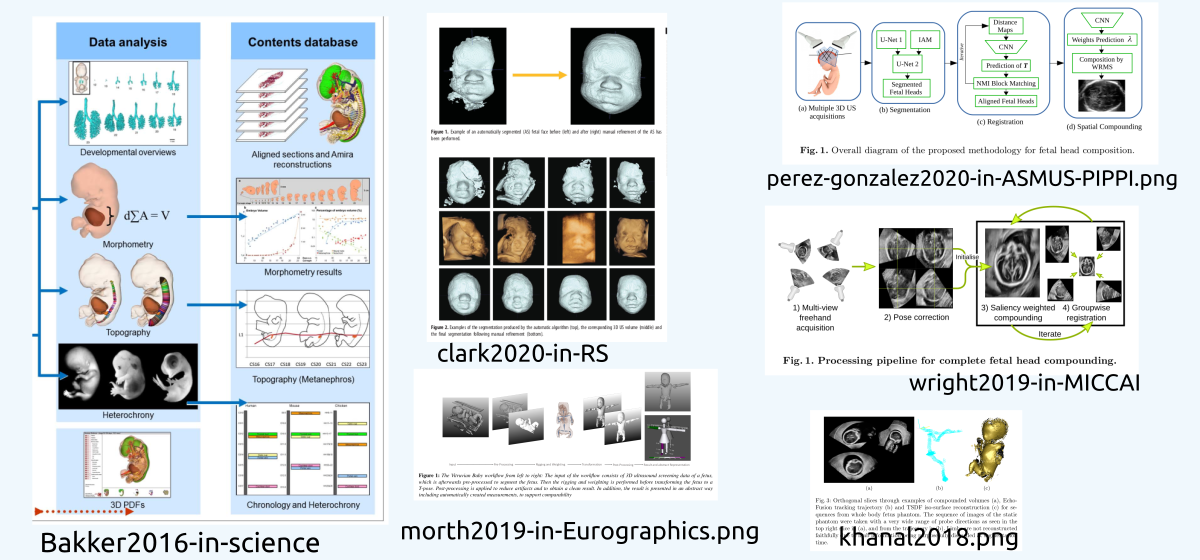
\includegraphics[width=1.0\textwidth]{state-of-the-art/versions/drawing-v01}
        %\caption{}
      \end{figure}
\end{frame}
}




% %%%%%%%%%%%%%%%%%%%%%%%%%%%%%%%%%%%%%%%%%%%%%%%%%%%%%%%%
% {
% %\paper{Wright-Gilbertson M. 2014 in PhD thesis}
% \begin{frame}{Fetal Biomechanics}
%       \begin{figure}
%         \centering
%         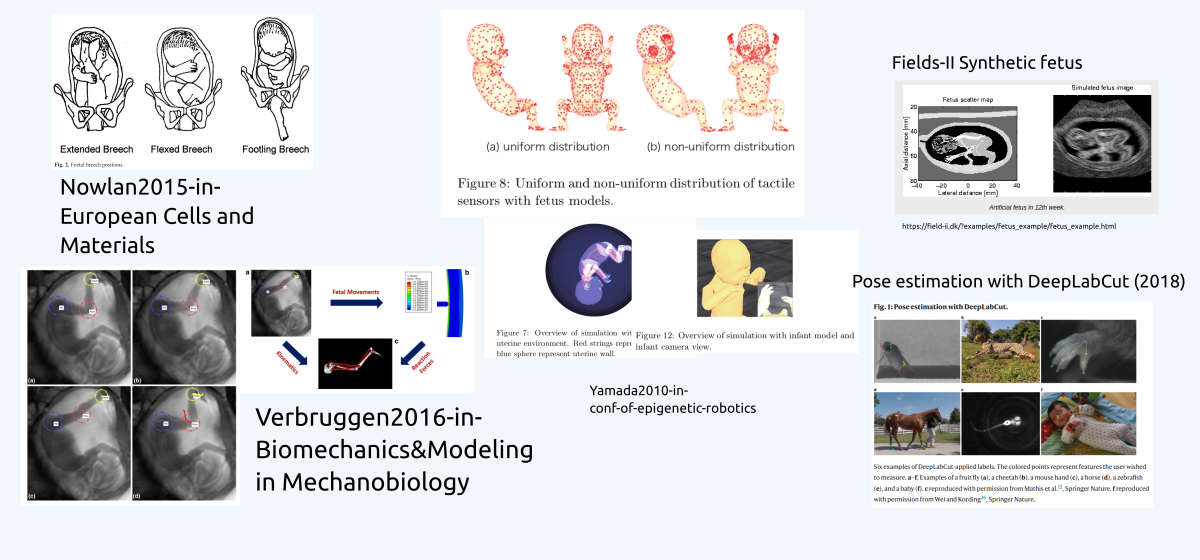
\includegraphics[width=1.0\textwidth]{fetal-biomechanics/versions/drawing-v00.png}
%         %\caption{}
%       \end{figure}
% \end{frame}
% }


% %%%%%%%%%%%%%%%%%%%%%%%%%%%%%%%%%%%%%%%%%%%%%%%%%%%%%%%%
% {
% %\paper{(a) Coordinate systems overview sketch in 3D Slicer,  (b) Asselin et al. 2018 in conf-BIVPCS, (c) US-simulator, and (d) 3D-printed fetus}
% %\paper{}
% \begin{frame}{Challenges of the fellowship}


%       \begin{figure}
%         \centering
%         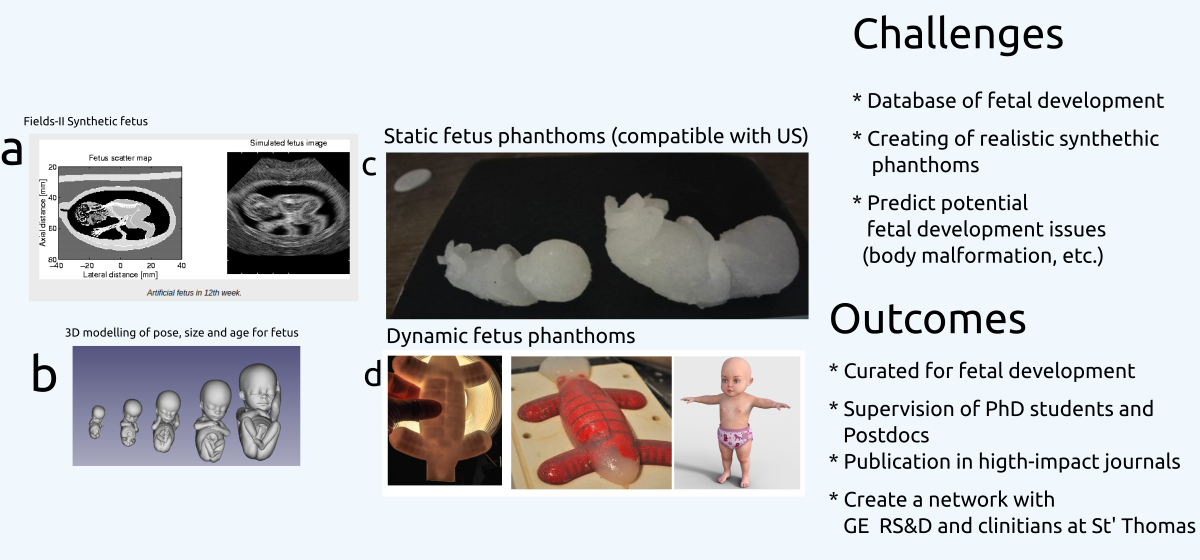
\includegraphics[width=1.0\textwidth]{simulator-for-ugi/versions/drawing-v02.png}
%       \end{figure}


% \end{frame}
% }




%%%%BLURS

% %%%%%%%%%%%%%%%%%%%%%%%%%%%%%%%%%%%%%%%%%%%%
% \subsection{Research Questions}


% %%%%%%%%%%%%%%%%%%%%%%%%%%%%%%%%%%%%%%%%%%%%%%%%%%%%%%%%
% {
% %\paper{Wright-Gilbertson M. 2014 in PhD thesis}
% \begin{frame}{Research Questions}	
%  %Can we understand more about fetal development trough the development of more realistic phantoms
% %Can dynamic fetal phantoms be created to understand fetal development?  %added Thu 15 Apr 05:20:09 BST 2021
% %Can synthetic fetus help to understand fetal development? %Fri 23 Apr 05:56:53 BST 2021
% %* Can the creation of synthetic fetuses help to understand fetal development? %Wed 12 May 08:20:58 BST 2021 
% %* Can the creation of synthetic fetuses predict fetal development issues? %Wed 12 May 09:50:47 BST 2021

% \BigSizeFont
% \begin{itemize}
% %\item Would the creation of synthetic fetuses help to understand 
% %the biomechatincs of phetal development? %Sat 15 May 14:51:42 BST 2021
% %\item Can we understand fetal development with synthetic fetuses? %Sat 15 May 15:08:19 BST 2021
% %\item Can the understanding of fetal biomechanics lead to predict fetal pathologies? %Mon 12 Jul 09:25:41 BST 2021
% % MORE ON FETAL PATHOLOGIES:https://www.sciencedirect.com/topics/medicine-and-dentistry/fetal-pathology
% \item Can fetal biomechanics help to understand the prediction of fetal pathologies? %% Mon 12/07/2021 09:45
% \item Would AI-based fetal biomechanics automatically predict fetal pathologies? %Tue 19 Oct 16:54:45 BST 2021
% \item \end{itemize}

% \end{frame}
% }


%\subsection{State-of-the-art on modelling fetus}




% \maketitle

\end{document}
